\documentclass[12pt,a4paper,oneside]{article}

\usepackage[left=3.5cm,top=3cm,right=2.5cm,bottom=3.5cm]{geometry}

\usepackage[english,italian]{babel}

\usepackage[usenames,dvipsnames,svgnames,table]{xcolor}

\usepackage{colortbl}

\usepackage{setspace}
\setstretch{1.35}

\usepackage{mathtools}

\usepackage[overload]{empheq}

\usepackage{amssymb}

\usepackage[bottom,marginal]{footmisc}
\setlength{\footnotemargin}{1.525em}

\usepackage[hidelinks]{hyperref}
\hypersetup{linktoc=all}

\usepackage{footnotebackref}

\usepackage{tablefootnote}

\usepackage[english,italian,nameinlink,capitalize]{cleveref}
\crefname{algocf}{algoritmo}{algoritmi}

\usepackage{graphicx}

\usepackage{tikz}
\usetikzlibrary{shapes,arrows,positioning}
\usepackage{pgfplots}
\pgfplotsset{compat=newest}

\usepackage{multirow}

\usepackage{array}

\usepackage{longtable}

\usepackage{calc}

\usepackage[hypcap=true,labelformat=simple]{subcaption}
\renewcommand\thesubfigure{(\alph{subfigure})}

\usepackage[algoruled,nofillcomment,vlined]{algorithm2e}

\usepackage{fancyhdr}
\pagestyle{fancy}
\fancyhf{}
\renewcommand{\headrulewidth}{0pt}
\fancyfoot[R]{\thepage}

\usepackage[nopostdot,nonumberlist]{glossaries}
\makeglossaries

\bibliographystyle{IEEEtran}

\author{Georgiu Gabriel Claudiu}
\title{RiskInDroid: analisi del rischio di applicazioni Android}

\newacronym{API}{API}{Application Programming Interface}
\newacronym{CVE}{CVE}{Common Vulnerabilities and Exposures}
\newacronym{CVSS}{CVSS}{Common Vulnerability Scoring System}
\newacronym{IDE}{IDE}{Integrated Development Environment}
\newacronym{IPC}{IPC}{Inter Process Communication}
\newacronym{NVD}{NVD}{National Vulnerability Database}
\newacronym{SVM}{SVM}{Support Vector Machines}
\newacronym{URL}{URL}{Uniform Resource Locator}





\begin{document}



\selectlanguage{italian}
\pagenumbering{Roman}
\thispagestyle{empty}
\begin{spacing}{1.3}
	\begin{center}
		\noindent\makebox[\textwidth][c]{\Large\bf UNIVERSITÀ DEGLI STUDI DI GENOVA}
		\noindent\makebox[\textwidth][c]{\large\bf Facoltà di Ingegneria}	
		
		\begin{figure}[!htb]
			\centering
			
\includegraphics[height=30mm]{resources/logo.png}
		\end{figure}
	
		\begin{minipage}[!htb]{\textwidth}
			\begin{singlespace}
				\begin{center}
					{\itshape Corso di Laurea Magistrale in Ingegneria Informatica} 
				\end{center}
			\end{singlespace}
		\end{minipage}
		
		\noindent\hrulefill\\
		
		\vfill
		
		\noindent\makebox[\textwidth][c]{
		\begin{minipage}[!htb]{.9\textwidth}
			\begin{center}
				{\LARGE\scshape RiskInDroid: analisi del rischio di applicazioni Android}
			\end{center}
		\end{minipage}}
	\end{center}
	
	\vfill
	
	\noindent\begin{minipage}[t]{\textwidth-5.9cm}
		\textit{Relatore:}
		\begin{singlespace}
			\textbf{Prof. Alessio MERLO}\\
		\end{singlespace}
	\end{minipage}%
	\noindent\begin{minipage}[t]{5.8cm}
		\textit{Candidato:}		
		\begin{singlespace}
			\textbf{Gabriel Claudiu GEORGIU}\\
			Matricola n. 3618343
		\end{singlespace}
	\end{minipage}%
	
	\vspace{2cm}
	
	\begin{center}
		\noindent\hrulefill\\
		\noindent\makebox[\textwidth][c]{Anno Accademico $2015  -  2016$}
	\end{center}	
\end{spacing}
\newpage



\selectlanguage{italian}
\begin{spacing}{1.6}
\setglossarystyle{altlist}
\printglossary[type=\acronymtype,title={Simboli e abbreviazioni}]
\end{spacing}
\newpage



\tableofcontents
\newpage

\listoffigures
\newpage
\listoftables
\newpage





\pagenumbering{arabic}
\section{Introduzione}\label{sec:Introduzione}

Con quasi $300$ milioni di smartphone venduti solamente nel secondo trimestre del $2016$ \cite{GARTNER}, Android risulta essere il sistema operativo per dispositivi mobili più diffuso al mondo e, di conseguenza, anche un bersaglio appetibile per gli autori di \textit{malware}, i quali possono sfruttare la sua popolarità per mettere in pericolo la privacy di milioni di utenti. È pertanto necessario prestare particolare attenzione agli aspetti di sicurezza legati alla piattaforma Android.

Con lo scopo di rendere l'utenza più consapevole del rischio in cui si incorre installando determinate applicazioni, questa tesi si prefigge l'obiettivo di proporre un metodo per l'analisi quantitativa del rischio delle app Android, volto a ricavare un punteggio numerico corretto ed affidabile che indichi quanto una certa app possa essere rischiosa. Dopo aver valutato due metodologie che si sono rivelate inadatte per una affidabile valutazione del rischio, viene ideato e proposto un nuovo metodo, denominato RiskInDroid, che si basa su tecniche di \textit{machine learning} per costruire un modello di rischio partendo da un ampio campione statistico raccolto specificatamente per questo lavoro di laurea, costituito da $116~541$ applicazioni benigne e $6~707$ \textit{malware}. Il funzionamento di RiskInDroid si fonda su un'analisi estensiva dei permessi delle applicazioni Android, e non soltanto sui permessi dichiarati (come nella maggior parte degli altri lavori scientifici), ma anche su quelli realmente utilizzati, richiesti ma non usati e infine utilizzati senza essere stati prima dichiarati.

Sebbene la letteratura scientifica che tratta argomenti riguardanti la sicurezza di Android sia molto vasta, finora si è focalizzata maggiormente sulla classificazione binaria di \textit{malware} e non sono presenti molti lavori incentrati sulla creazione di un indice di rischio quantitativo. Le metodologie basate sulla classificazione binaria hanno il limite intrinseco di non poter fornire alcun valore quantitativo riferito alla pericolosità di un'app; per quanto riguarda invece le tecniche già proposte per la valutazione del rischio, alcune non sono applicabili in generale perché necessitano di conoscere la categoria di appartenenza dell'applicazione \cite{ROTARU,CATEGORICAL_RISK}, mentre in altri casi i valori di rischio non sono facilmente confrontabili perché non è stato fissato un intervallo limitato entro cui far variare tali valori \cite{WANG_QUANTITATIVE}. RiskInDroid, il metodo proposto in questa tesi, prende spunto dalle metodologie basate sulla classificazione binaria di \textit{malware}, integrando però le intuizioni più interessanti presenti nelle pubblicazioni riguardanti l'analisi di rischio delle applicazioni. In questo modo si ottiene un approccio applicabile in maniera generale e un indice di rischio facilmente interpretabile e confrontabile con gli indici di rischio di altre app, superando dunque le limitazioni dei metodi proposti finora.

Per quanto riguarda la realizzazione pratica di RiskInDroid, si è deciso di impiegare il linguaggio di programmazione Python, scelta dettata soprattutto dalla volontà di utilizzare la libreria \mbox{\textit{scikit-learn}}~\cite{SCIKIT}, che implementa le tecniche di \textit{machine learning} necessarie al funzionamento di RiskInDroid. Una volta completato lo sviluppo e dopo aver valutato empiricamente l'efficacia del metodo, RiskInDroid è stato integrato come componente di Approver \cite{APPROVER}, un \textit{tool} professionale per l'analisi completa delle applicazioni mobili sviluppato da Talos S.r.l.s (\url{http://www.talos-security.com/}) in collaborazione con il Computer Security Lab del dipartimento DIBRIS dell'Università di Genova.



\subsection{Organizzazione della tesi}
La tesi è organizzata secondo l'ordine cronologico di svolgimento: si inizia con una presentazione complessiva del lavoro che si intende compiere, si prosegue illustrando metodologie e strumenti impiegati per concludere infine con l'analisi e il commento dei risultati ottenuti, indicandone eventuali sviluppi futuri.

La \hyperref[sec:Introduzione]{Sezione introduttiva} offre una panoramica generale sugli argomenti trattati in questa tesi ed espone gli obiettivi prefissati.

La \cref{sec:Android} presenta in maniera sintetica l'architettura del sistema operativo Android, con particolare attenzione al meccanismo di sicurezza basato sull'utilizzo di permessi e menzionando i principali canali di distribuzione delle app.

La \cref{sec:Stato_arte} mostra i risultati più importanti ottenuti finora dalla comunità scientifica nell'ambito della classificazione binaria di \textit{malware} e dell'analisi quantitativa del rischio delle applicazioni Android. Viene inoltre brevemente descritta la libreria di Python che implementa le tecniche di \textit{machine learning} adoperate nel corso della tesi.

Nella \cref{sec:Metodologia} viene esposta nel dettaglio la metodologia adottata in questo elaborato di laurea: inizialmente viene proposto un approccio per l'analisi del rischio delle applicazioni basato sull'elenco \acrshort{CVE}, che si rivela tuttavia poco funzionale; si valutano pertanto due ulteriori metodi, il secondo dei quali, denominato RiskInDroid, ha un carattere innovativo e risulta efficace nell'utilizzo pratico.

La \cref{sec:Risultati} riporta i risultati ottenuti sperimentalmente applicando il metodo RiskInDroid su un campione statistico costituito da oltre $100~000$ applicazioni Android. Le app valutate con un indice di rischio elevato vengono successivamente analizzate con una suite di antivirus online per determinarne la reale pericolosità.

Nella \hyperref[sec:Conclusioni]{Sezione conclusiva} vengono fatte alcune considerazioni sui risultati ottenuti durante lo svolgimento della tesi, illustrando infine alcuni spunti per proseguire ulteriormente il lavoro iniziato in questo elaborato di laurea.
\newpage





\section{Ecosistema Android}\label{sec:Android}

Android è un sistema operativo per dispositivi mobili \textit{open source} basato su \textit{kernel} Linux, sviluppato da Google e dall'Open Handset Alliance. È composto da un'architettura a più livelli di astrazione\footnote{\url{http://developer.android.com/guide/platform/index.html}}, come visibile in \cref{fig:android_stack}.

\begin{figure}[!htb]
    \centering
    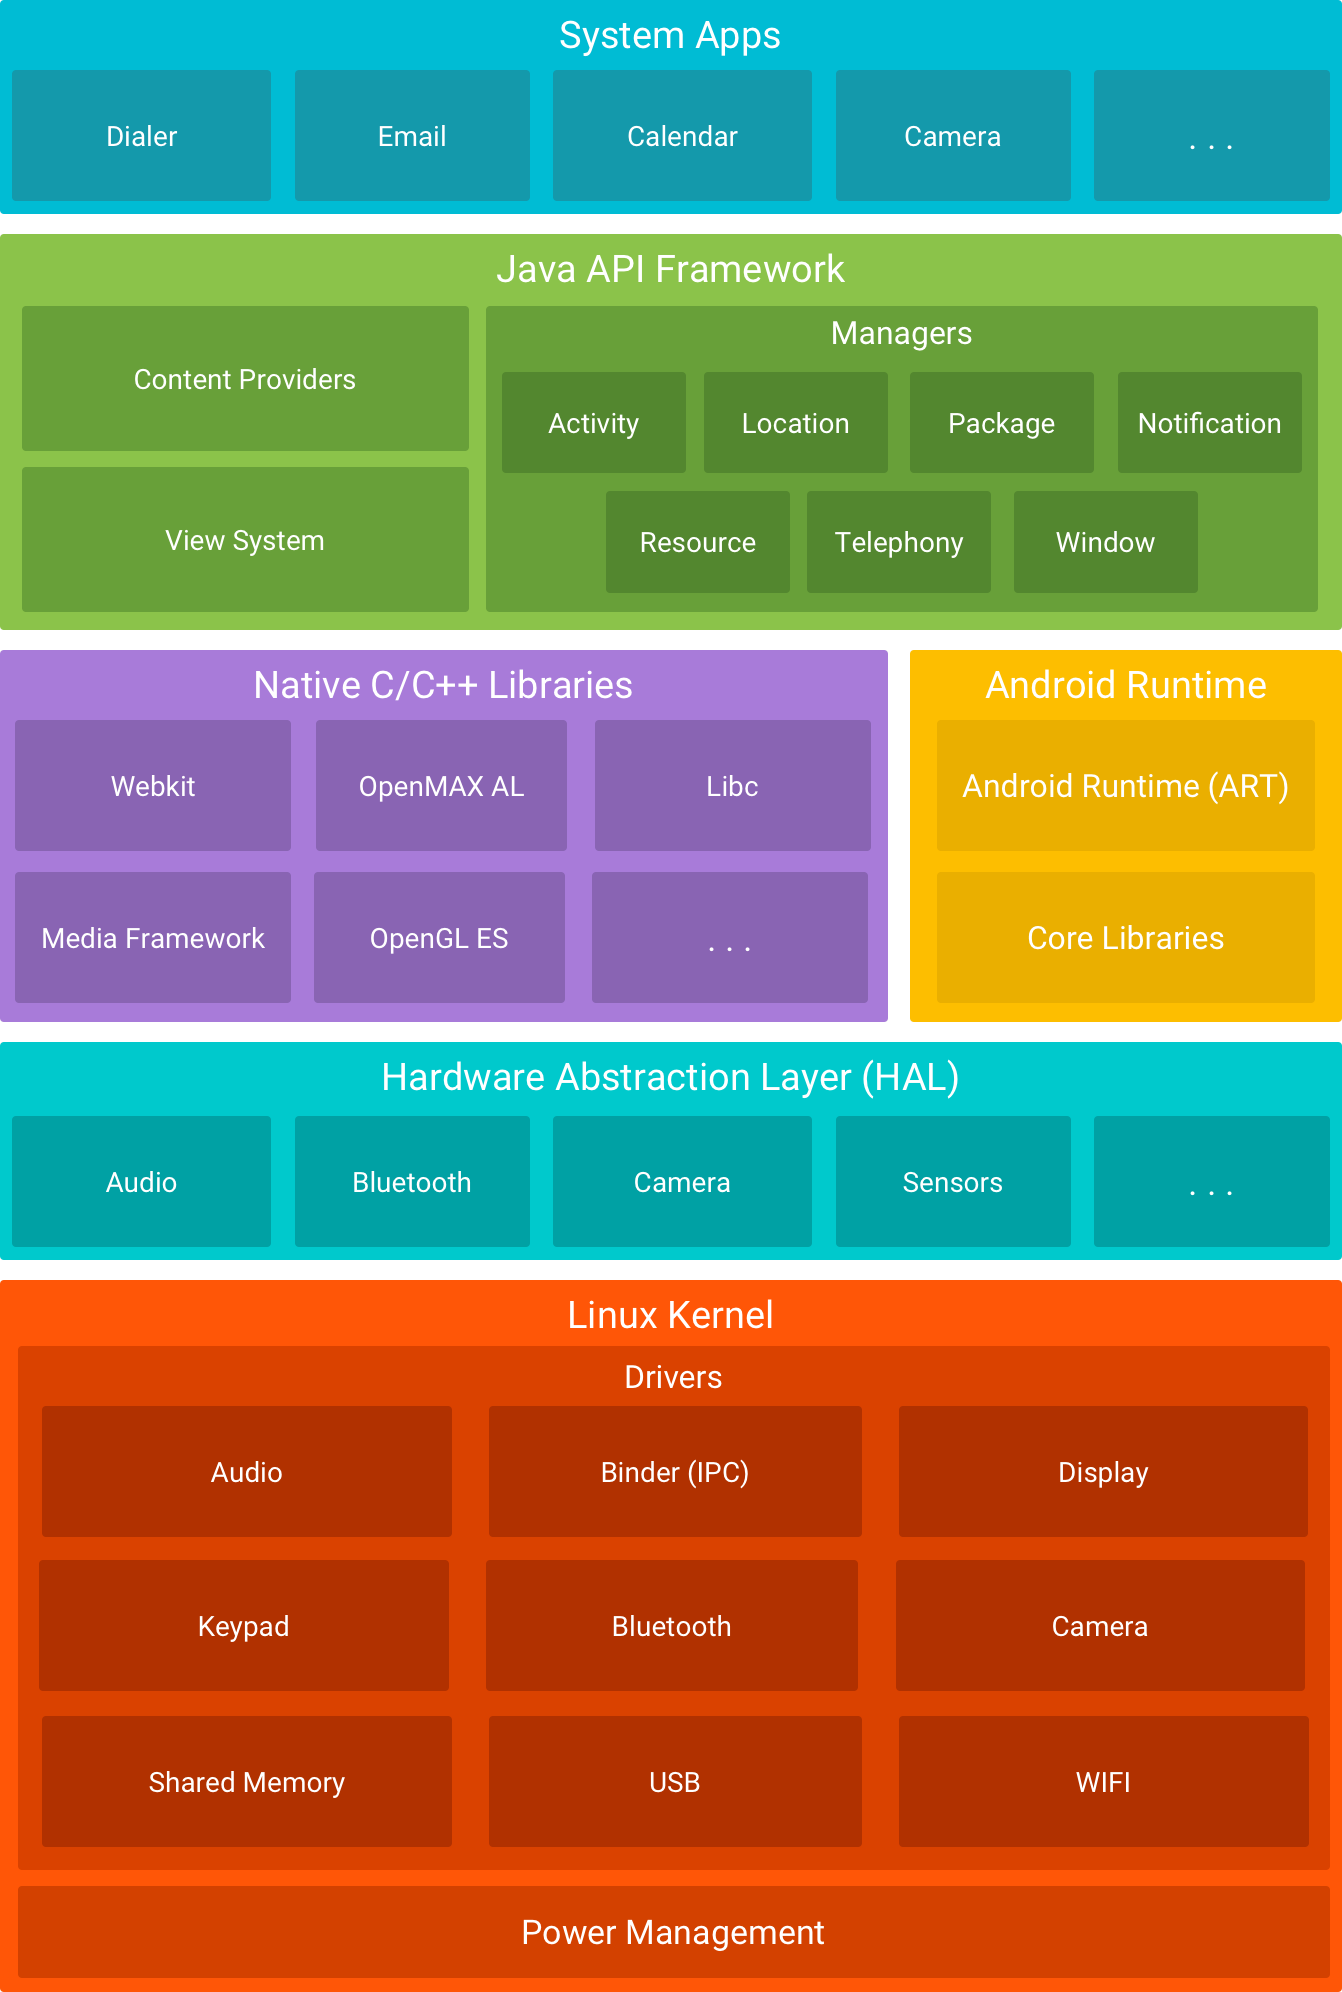
\includegraphics[height=16cm]{resources/images/android_stack.png}
    \caption{Architettura a livelli della piattaforma Android}\label{fig:android_stack}
\end{figure}

\noindent In cima allo \textit{stack} dell'architettura di Android si trovano le \textbf{applicazioni di sistema} che offrono le funzionalità di base (gestione email, calendario ecc.). Al livello appena inferiore è presente il \textbf{Java \acrshort{API} framework}, che fornisce un set di componenti modulari riutilizzabili per lo sviluppo di nuove applicazioni in linguaggio Java, come ad esempio funzioni per accedere alle risorse o per mostrare notifiche nella barra di stato dell'app. Il sistema Android rende inoltre disponibile l'accesso a \textbf{librerie native} scritte in \mbox{C/C++} tramite l'impiego di Android NDK (\textit{Native Development Kit}), nel caso si vogliano ottenere prestazioni più elevate nelle operazioni che coinvolgono l'impiego di grafica $2$D e $3$D. L'\textbf{Android Runtime} è il livello dove vengono eseguite più istanze di macchine virtuali (una per ogni applicazione) ottimizzate per avere un basso consumo di risorse. In particolare, ogni macchina virtuale esegue il \texttt{DEX} \textit{bytecode} generato a partire dall'app scritta in Java. L'\textbf{Hardware Abstraction Layer} è formato da un insieme di librerie che rende possibile l'utilizzo delle risorse hardware da parte del livello superiore (Java \acrshort{API} framework). Alla base di tutta l'architettura è presente il \textbf{Kernel Linux}, che astrae l'hardware del dispositivo e fornisce funzionalità elementari, ad esempio per la gestione dei processi, della memoria o dell'\textit{\gls{IPC}}.

Il sistema operativo Android assegna ad ogni applicazione un Linux \texttt{user ID} univoco in fase di installazione della stessa. In combinazione al fatto che ogni app viene eseguita in una propria istanza di macchina virtuale, ciò contribuisce alla creazione di una \textit{sandbox} che garantisce l'isolamento di ogni applicazione installata rispetto alle altre e rispetto al sistema operativo. Android implementa dunque il principio del minimo privilegio\footnote{\url{http://developer.android.com/guide/components/fundamentals.html}}, pertanto ogni app che voglia accedere a risorse protette del dispositivo (fotocamera, memoria esterna ecc.) oppure a dati di altre applicazioni deve richiedere esplicitamente l'autorizzazione all'utente. Questo meccanismo di autorizzazione viene garantito in Android tramite l'utilizzo di permessi. Nelle versioni di Android precedenti alla $6.0$, i permessi sono richiesti in fase di installazione dell'app e l'utente deve accettarli tutti affinché l'installazione venga completata; nelle versioni successive i permessi sono invece gestiti dinamicamente (ovvero sono richiesti quando vengono utilizzati)\footnote{\url{http://developer.android.com/training/permissions/requesting.html}}.



\subsection{Sistema dei permessi in Android}

Il sistema dei permessi è uno dei principali meccanismi di sicurezza su cui si basa Android. Ogni app viene infatti eseguita in un processo isolato ed è grazie ai permessi che le vengono concessi che può accedere a specifiche risorse del sistema. I permessi sono dichiarati nel file \texttt{AndroidManifest.xml}, che contiene anche altre informazioni fondamentali riguardanti l'applicazione come il ad esempio il suo nome, le versioni di Android compatibili e tutti i componenti presenti nell'app. Al momento della stesura della tesi, il sistema operativo Android mette a disposizione più di $130$ permessi\footnote{\url{http://developer.android.com/reference/android/Manifest.permission.html}}; gli sviluppatori possono tuttavia definire nuovi permessi (ad esempio per esporre in maniera controllata funzionalità delle proprie app verso l'esterno) o richiedere permessi specifici dichiarati da altre applicazioni. I permessi inclusi nel sistema Android sono classificati in $4$ categorie\footnote{\url{http://developer.android.com/guide/topics/manifest/permission-element.html}} in base al loro rischio potenziale:
\begin{enumerate}
    \item[1)]\texttt{normal}: tipologia di permesso utilizzata di default che viene concessa all'applicazione direttamente dal sistema senza notificare l'utente. Si tratta di permessi per accedere a risorse a basso rischio;
    \item[2)]\texttt{dangerous}: categoria di permessi più rischiosi del normale, generalmente non necessari per le applicazioni, ma richiesti per accedere ai dati privati e all'hardware del dispositivo (ad esempio, per leggere i contatti o per effettuare chiamate). Tali permessi possono essere concessi solamente tramite la conferma esplicita dell'utente;
    \item[3)]\texttt{signature}: questi permessi possono essere concessi solamente ad applicazioni firmate con lo stesso certificato di quelle che hanno dichiarato i permessi e, in caso la firma coincida, sono concessi senza bisogno di notificare l'utente;
    \item[4)]\texttt{signatureOrSystem}: tipologia di permesso speciale garantita in modo automatico alle applicazioni incluse nell'immagine di sistema Android.
\end{enumerate}



\subsection{\textit{Application Store}}

Il successo e la diffusione di un sistema operativo sono fortemente influenzati dalla quantità di programmi e/o applicazioni disponibili. Rispetto alla concorrenza, Android è avvantaggiato dal fatto di essere \textit{open source} e perché, modificando una semplice impostazione, permette di installare app da fonti non ufficiali. Per questo motivo, oltre al Google Play Store, sono presenti svariati \textit{application store} alternativi da dove è possibile scaricare ed installare app per il proprio dispositivo mobile, come ad esempio Aptoide e Uptodown. In questa tesi vengono dunque presi in considerazione sia canali di distribuzione ufficiali (ad esempio Google Play Store, Samsung Store ecc.) sia fonti non ufficiali (come siti web, \textit{market} non ufficiali ecc.) per disporre di un campione statistico sufficientemente ampio per una valutazione affidabile dell'approccio proposto in questa tesi per l'analisi del rischio di app Android.
\newpage





\section{Stato dell'arte}\label{sec:Stato_arte}

Al giorno d'oggi Android è un sistema operativo installato sull'$86.2\%$ dei dispositivi mobili \cite{GARTNER}, con centinaia di migliaia di applicazioni disponibili (e non sempre provenienti da fonti ufficiali), pertanto il problema della sicurezza su questa piattaforma è molto attuale. Negli ultimi anni la comunità scientifica, e non solo, ha proposto diverse metodologie allo scopo di individuare le caratteristiche ed i comportamenti che contraddistinguono i \textit{malware} (app malevole) dalle app benigne. In particolare, esistono due approcci generali per il rilevamento di applicazioni malevole: analisi statica e dinamica. Le tecniche basate sull'analisi statica consistono nell'esaminare il codice sorgente decompilato, senza eseguire l'applicazione; in questo modo è possibile estrarre informazioni per individuare, ad esempio, i permessi, i \textit{broadcast receiver} oppure la presenza di stringhe sospette. Nel caso di analisi dinamica, l'app viene invece eseguita in un ambiente di test controllato per monitorarne il comportamento, ed è possibile ottenere dati riguardanti il traffico di rete generato o le risorse di sistema utilizzate. Generalmente, entrambi i tipi di analisi prevedono la creazione di un modello di classificazione a partire dalle informazioni osservate, in modo da riuscire a distinguere le applicazioni benigne da quelle maligne in base alle loro caratteristiche, codificate come \textit{feature}.

In questo elaborato di laurea ci si concentra solamente sui metodi di analisi statica, in particolare su quelli basati sui permessi relativi alle app Android, senza indagare su metodologie che ricorrono all'analisi dinamica (ad esempio \cite{CROWDROID}): come dimostra infatti la letteratura scientifica (\cref{sec:classificazione_binaria,sec:risk_analysis}), impiegando metodologie incentrate sull'analisi statica si ottengono spesso buoni risultati e non è necessario investire risorse in dispositivi mobili e/o emulatori (indispensabili per l'analisi dinamica). Nello specifico, si è partiti esaminando i lavori presenti nella letteratura scientifica riguardanti la classificazione binaria di \textit{malware} e quelli relativi alla creazione di un punteggio di rischio per le applicazioni Android. Dopodiché, dall'analisi dello stato dell'arte di queste due branche di ricerca è stato proposto un approccio nuovo (RiskInDroid) per la generazione di un indice di rischio per app Android.



\subsection{Classificazione binaria di \textit{malware}}\label{sec:classificazione_binaria}

Le pubblicazioni scientifiche che trattano il problema della classificazione binaria di \textit{malware} in ambito Android sono numerose. Vengono analizzate di seguito solo quelle più rilevanti e promettenti ai fini dell'obiettivo di questa tesi.
\newline

Uno dei primi lavori proposti allo scopo di individuare i \textit{malware} in maniera semplice ed efficiente è Kirin \cite{KIRIN}. Si tratta di un elenco di regole di sicurezza che descrivono pattern considerati pericolosi a partire dalle informazioni reperibili nel file \texttt{AndroidManifest.xml} delle app Android. Ad esempio, è considerata pericolosa un'app che richieda contemporaneamente i permessi \texttt{RECEIVE\_SMS} e \texttt{WRITE\_SMS}. Questa tecnica viene valutata su un totale di $311$ applicazioni popolari scaricate dal Google Play Store nel $2009$, individuando $10$ app che violano la tutte le regole predefinite, di cui $5$ risultano effettivamente sospette anche dopo un'analisi manuale più approfondita.
\newline

Gli autori di \cite{PERMISSION_FEATURES} suggeriscono una metodologia basata sul \textit{machine learning} per riconoscere i \textit{malware}, utilizzando come algoritmi \textit{k-means} e gli alberi decisionali. Da ogni applicazione analizzata viene estratto un vettore di \textit{feature} formato da $0$ e $1$, riguardante soprattutto i permessi richiesti dall'app, dove $1$ indica la richiesta dello specifico permesso e $0$ l'assenza; questo modo di costruire le \textit{feature} viene adottato anche in RiskInDroid. Il metodo sviluppato in \cite{PERMISSION_FEATURES} viene validato con un \textit{dataset} di $500$ applicazioni ottenendo buoni risultati.
\newline

In \cite{PUMA} viene presentato un lavoro simile a \cite{PERMISSION_FEATURES}, in quanto si utilizzano tecniche di \textit{machine learning} su insiemi di \textit{feature} estratte dal file \texttt{AndroidManifest.xml} delle applicazioni Android (in particolare i permessi dichiarati). Con a disposizione un \textit{dataset} composto da $249$ \textit{malware} e $357$ app benigne, in \cite{PUMA} si valutano le prestazioni di diversi classificatori nell'individuare le app malevole, fra cui alberi decisionali, \textit{Random Forest} e \textit{Naive Bayes}.
\newline

Gli autori di \cite{TWO_LAYER} sviluppano una metodologia basata non solo sui permessi dichiarati dalle app Android, ma anche su quelli effettivamente utilizzati. Inoltre, per la creazione dei vettori di \textit{feature}, non vengono considerati solamente i singoli permessi, ma anche le coppie di permessi (sia dichiarati sia realmente utilizzati). La tecnica proposta è articolata in due fasi sequenziali in cui si controllano inizialmente i permessi richiesti e poi le coppie di permessi effettivamente utilizzati. Empiricamente si ottengono ottimi risultati, impiegando come classificatore gli alberi decisionali e conducendo i test su un insieme di $20~548$ applicazioni benigne e $1~136$ \textit{malware}.
\newline

In \cite{DREBIN_DATASET} viene proposto DREBIN, un metodo efficiente per il riconoscimento di \textit{malware} tramite analisi statica. A partire dal file \texttt{AndroidManifest.xml} e dal codice decompilato delle app, vengono estratti insiemi di \textit{feature} sottoposti ad un classificatore formato da \textit{Support Vector Machines} (\acrshort{SVM}). Questo metodo viene testato su un insieme di $123~453$ applicazioni benigne e $5~560$ \textit{malware}, ottenendo risultati che indicano un'accuratezza del $94\%$, con solo l'$1\%$ di falsi positivi. Questa metodologia può essere impiegata anche direttamente sui dispositivi mobili, con tempi di esecuzione nell'ordine di alcuni secondi. Per ogni app esaminata, DREBIN fornisce inoltre una descrizione delle \textit{feature} sospette individuate. La collezione di \textit{malware} utilizzata in \cite{DREBIN_DATASET} viene resa disponibile come DREBIN \textit{dataset} e viene impiegata anche per le prove empiriche utilizzate per la validazione sperimentale di RiskInDroid.



\subsection{Analisi del rischio}\label{sec:risk_analysis}

La letteratura scientifica riguardante l'analisi del rischio delle applicazioni Android contiene un numero inferiore di pubblicazioni rispetto a quella relativa alla classificazione binaria di \textit{malware}; pertanto, nel seguito di questa sezione sono presentati i principali lavori scientifici che prevedono metodi quantitativi per la valutazione del rischio delle app Android.
\newline

In \cite{ROTARU} è descritto un metodo per rilevare segnali di rischio per le applicazioni in base a quanto raramente vengono richiesti permessi (o coppie di permessi) critici, dove con permesso critico si intende un permesso con un impatto significativo per la sicurezza e/o per la privacy dell'utente. In particolare, se un'app richiede un permesso che è poco presente nelle altre app della stessa categoria, tale app è considerata rischiosa. Sempre in \cite{ROTARU} viene indicato come ottenere alcune funzioni per il calcolo del rischio delle applicazioni Android, basandosi su modelli probabilistici bayesiani; tuttavia, per poter applicare questi metodi, è necessario conoscere anche la categoria di appartenenza dell'app (informazione reperibile nello \textit{store} da cui viene scaricata l'app, come ad esempio Giochi, Musica, Produttività ecc.). Vengono inoltre menzionate $3$ proprietà interessanti che dovrebbe avere ogni funzione per la generazione di un punteggio di rischio:
\begin{enumerate}
    \item[1)]\textbf{monotonicità}, rimuovendo un permesso richiesto da un'applicazione, il valore di rischio della stessa dovrebbe diminuire;
    \item[2)]\textbf{coerenza}, le app maligne dovrebbero avere un indice di rischio alto;
    \item[3)]\textbf{facilità di comprensione}, in modo che il valore di rischio di un'applicazione sia facilmente interpretabile e confrontabile con altre applicazioni.
\end{enumerate}
Le prove empiriche in \cite{ROTARU} sono eseguite su un \textit{dataset} composto da due insiemi di applicazioni benigne costituiti rispettivamente da $71~331$ e $136~534$ campioni, raccolti nel $2011$ e nel $2012$, e da una collezione di $808$ \textit{malware}.
\newline

In \cite{CATEGORICAL_RISK} viene suggerito un approccio per calcolare il rischio delle app Android basandosi sulla loro categoria di appartenenza. Nello specifico, una volta creati i vettori di \textit{feature} a partire dai permessi richiesti dalle applicazioni, per ogni categoria si determinano quali e quanti sono i permessi più richiesti dalle app benigne presenti in quella categoria, individuando in tal modo i pattern di permessi per ogni categoria. A questo punto è possibile calcolare un indice di rischio per una nuova applicazione andando a misurare quanto i permessi richiesti dall'app si discostano dai pattern rilevati in precedenza. Nonostante i buoni risultati ottenuti empiricamente su un \textit{dataset} formato da $7~737$ app benigne e $1~260$ \textit{malware}, il limite maggiore di questo metodo consiste nella necessità di conoscere la categoria di appartenenza delle applicazioni, informazione non sempre disponibile o affidabile.
\newline

In \cite{MULTILAYER_RISK} viene descritto un \textit{framework} di valutazione del rischio per le applicazioni composto di $3$ livelli interdipendenti: analisi statica, analisi dinamica e analisi comportamentale. Ogni livello si occupa di aspetti specifici dell'applicazione ed è il \textit{framework} proposto a combinare i risultati ricavati dai singoli moduli in modo da ottenere il rischio associato all'applicazione, il quale è composto da informazioni dettagliate come un punteggio di rischio numerico e una lista di fattori determinanti che rendono l'app rischiosa. Il \textit{framework} presentato è descritto nel dettaglio ma solamente in maniera teorica, in quanto in \cite{MULTILAYER_RISK} non vengono riportate prove empiriche a sostegno della metodologia proposta.
\newline

Gli autori di \cite{WANG_QUANTITATIVE} realizzano DroidRisk, un metodo quantitativo per il calcolo di un indice di rischio per le applicazioni Android. Disponendo di una collezione formata da $27~274$ app benigne e $1~260$ app maligne, in \cite{WANG_QUANTITATIVE} vengono presentate alcune statistiche relative ai permessi delle applicazioni nel \textit{dataset} e successivamente viene descritta una formula probabilistica, costituita dal prodotto fra la probabilità di richiesta e fra l'impatto di ogni permesso (inteso come il danno potenziale che si può causare utilizzando tale permesso). Questo metodo viene approfondito più nel dettaglio nella \cref{sec:probabilistic_method} di questa tesi.



\subsection{Libreria \mbox{\textit{scikit-learn}}}

\mbox{\textit{Scikit-learn}}~\cite{SCIKIT} (\url{http://scikit-learn.org/}) è una libreria \textit{open source} sviluppata in linguaggio Python che contiene le implementazioni dei principali algoritmi di \textit{machine learning} per la risoluzione di problemi di classificazione, regressione e \textit{clustering}. Lo scopo di questa libreria non è concentrarsi sul numero di funzionalità offerte, ma di fornire algoritmi implementati allo stato dell'arte, con particolare attenzione alla qualità del codice sorgente sviluppato. In \cite{SCIKIT_API} si può trovare una descrizione più approfondita della struttura interna della libreria; qui di seguito ci si limita a discutere le motivazioni che rendono \mbox{\textit{scikit-learn}} adatta per l'obiettivo di questa tesi.

Il motivo principale per la scelta di impiegare \mbox{\textit{scikit-learn}} è la presenza della funzione \texttt{predict\_proba} nella maggior parte dei classificatori resi disponibili dalla libreria. Si tratta di una funzione che, invece di restituire solamente il nome della classe predetta, indica in output la probabilità con cui ogni classe viene predetta dai metodi di classificazione. Per alcuni classificatori, come \textit{Naive Bayes}, ottenere le probabilità di ogni classe è immediato perché sono i classificatori stessi ad essere probabilistici; in altri casi è invece possibile ricavare le probabilità delle classi predette utilizzando le tecniche descritte in \cite{GET_PROBABILITIES}, come viene fatto ad esempio per le \textit{Support Vector Machines}.

\mbox{\textit{Scikit-learn}} è dunque una libreria potente e versatile, ma anche relativamente semplice da utilizzare per gli utenti meno esperti. Presenta tuttavia dei limiti per quanto riguarda l'esecuzione parallela di codice che sfrutti la presenza di più processori di calcolo; inoltre non è stata ancora realizzata una soluzione stabile e duratura per il salvataggio in maniera persistente dei modelli di classificazione, una volta eseguito il \textit{training} (operazione che può rivelarsi costosa in termini di tempo).
\newpage





\section{Metodologia}\label{sec:Metodologia}

Per l'implementazione dei metodi proposti in questo elaborato di laurea vengono utilizzati principalmente due strumenti di sviluppo. Inizialmente, per il lavoro di tesi viene impiegato l'\gls{IDE} IntelliJ IDEA $2016$\footnote{\hspace{.175em}\url{http://www.jetbrains.com/idea/}} e il linguaggio di programmazione Java, con cui viene scritto il codice relativo alla \cref{sec:cve}. Successivamente, per poter far uso della libreria di \textit{machine learning} chiamata \mbox{\textit{scikit-learn}}, si passa al linguaggio Python, adoperando come \textit{editor} Visual Studio Code\footnote{\hspace{.175em}\url{http://code.visualstudio.com}}. Trattandosi di strumenti multi-piattaforma, durante lo svolgimento della tesi vengono utilizzati sia il sistema operativo Windows~$10$ sia Ubuntu~$16.04$ (eseguito in una macchina virtuale).



\subsection{Raccolta delle applicazioni}\label{sec:dataset}

Per la valutazione della qualità dei metodi proposti e delle relative implementazioni, è prima di tutto necessario costruire una base di dati che contenga un buon numero di campioni da analizzare.

\begin{table}[!htb]
    \renewcommand{\arraystretch}{1.3}
    \centering
    \begin{tabular}{|>{\centering\arraybackslash}m{.4\textwidth}||>{\centering\arraybackslash}m{.4\textwidth}|}
        \hline
        Fonte & Numero di applicazioni\\
        \hline\hline
        Raccolta \textit{malware} & $\hspace{1em}6~707$\\\hline
        Google Play Store\tablefootnote{\url{http://play.google.com/store/apps}} & $101~730$\\\hline
        Aptoide\tablefootnote{\url{http://www.aptoide.com/page/apps}} & $\hspace{1em}7~609$\\\hline
        Uptodown\tablefootnote{\url{http://en.uptodown.com/android}} & $\hspace{1em}7~202$\\\hline\hline
        Totale & $123~248$\\\hline
    \end{tabular}
    \caption{Composizione del \textit{dataset} di applicazioni}
    \label{tab:APK_dataset}
\end{table}

\noindent Nella \cref{tab:APK_dataset} è visibile l'origine delle applicazioni prese in esame durante questo elaborato di laurea. L'insieme di \textit{malware} è costituito principalmente dal DREBIN \textit{dataset}~\cite{DREBIN_DATASET} ($5~560$ campioni), con l'aggiunta di ulteriori elementi ottenuti da risorse liberamente accessibili online \cite{CONTAGIO_DATASET, HUSTED_DATASET, BHATIA_DATASET}. I campioni restanti vengono invece scaricati dai relativi \textit{app store} mediante un \textit{crawler} creato ad hoc; dato che il Google Play Store è il canale ufficiale per ottenere applicazioni per dispositivi Android, queste vengono considerate (solo inizialmente) non malevole\footnote{La collezione di applicazioni provenienti dal Google Play Store viene analizzata nella \cref{sec:Risultati} per determinare se contiene o meno campioni appartenenti alla categoria \textit{malware}\vspace{1ex}}. A causa della natura eterogenea delle fonti, ad ogni app viene associato un codice univoco di $32$ cifre esadecimali, chiamato \textit{hash MD5}, per evitare di avere duplicati.

Prendere in considerazione una quantità elevata di dati da analizzare (come fatto per il \textit{dataset} di questa tesi) è importante perché permette di ottenere risultati che valgono in generale e non solo in casi specifici, con il vantaggio di avere una maggiore disponibilità di elementi su cui testare gli algoritmi proposti. Tuttavia, a causa del numero relativamente basso di \textit{malware} nel \textit{dataset}, per condurre prove empiriche, vengono estratti in modo pseudo-casuale $3$ insiemi distinti dalle applicazioni scaricate dal Google Play Store che abbiano la stessa dimensione della raccolta di \textit{malware}, impiegando la funzione \texttt{random.sample}\footnote{\url{http://docs.python.org/3/library/random.html\#random.sample}} presente in Python e fissando il parametro \texttt{random.seed} in modo da avere sempre risultati riproducibili. Pertanto, ognuno dei $3$ set ricavati è formato per metà dalla collezione di applicazioni maligne e per l'altra metà da un insieme di app benigne provenienti dal Google Play Store; in questo modo ogni set creato contiene al suo interno un numero bilanciato di \textit{malware} e di applicazioni non malevole.



\subsection{\textit{\acrlong{CVE}}}\label{sec:cve}

Un primo tentativo di creare un punteggio di rischio è stato fatto utilizzando il \textit{\gls{CVE}}, un database liberamente consultabile online all'indirizzo web \url{http://cve.mitre.org/} contenente informazioni di dominio pubblico su falle di sicurezza e vulnerabilità note relative ai sistemi informatici. In particolare, per gli scopi di questo elaborato, si era interessati esclusivamente alle \textit{entry} collegate all'ecosistema Android. A ogni voce inserita nel \gls{CVE} è assegnato un codice in formato \texttt{CVE-[anno]-[numero progressivo]} (ad esempio \texttt{CVE-$2016$-$3897$}) che identifica in modo univoco una vulnerabilità. Tramite questo codice è possibile reperire ulteriori informazioni dal \textit{\gls{NVD}}, sito gestito dal governo degli Stati Uniti\footnote{\url{http://nvd.nist.gov/}}. Nello specifico, si possono ottenere dettagli tecnici come la classe a cui appartiene la vulnerabilità, le configurazioni di software esposte al rischio, le competenze necessarie per sfruttare la falla e soprattutto un punteggio numerico fra $0.0$ e $10.0$ che ne indica la gravità, chiamato \textit{\gls{CVSS}}\footnote{\url{http://www.first.org/cvss}}.

Al momento della stesura della tesi, consultando il \gls{CVE} si possono trovare circa $2~500$ voci relative ad Android. Una prima strada esplorata per l'ottenimento di un indice di rischio per le applicazioni è quindi la seguente: per ogni app analizzata, si scorre l'elenco delle vulnerabilità del \gls{CVE} collegate ad Android, controllando di volta in volta se la descrizione della falla di sicurezza è in qualche modo riconducibile all'applicazione in esame o a un suo componente. Se si riescono a trovare una o più vulnerabilità, queste vengono assegnate all'app e, grazie al loro identificativo univoco, è possibile estrarne il punteggio \gls{CVSS} da cui ottenere infine l'indice di rischio desiderato. La fase cruciale e più difficile di questo metodo è riuscire a fare il \textit{mapping} fra la descrizione in linguaggio naturale della vulnerabilità e l'applicazione stessa o un suo componente.

Analizzando più nel dettaglio l'elenco \gls{CVE} inerente ad Android, si possono individuare più categorie di vulnerabilità:
\begin{enumerate}
    \item[a)]Problemi relativi alla verifica dei certificati SSL X.$509$. Si tratta di vulnerabilità che affliggono versioni specifiche di determinate applicazioni e costituiscono circa il $56\%$ della lista \gls{CVE} considerata. Questo gruppo di problemi non può essere utilizzato per la creazione di un indice di rischio generale perché è riferito a versioni specifiche di app, che con buona probabilità avranno già corretto il baco nella \textit{release} immediatamente successiva;
    \item[b)]Vulnerabilità inerenti soltanto determinate applicazioni, quindi non utilizzabili per la costruzione di un punteggio di rischio generale. Ad esempio, sommando i problemi relativi ad Adobe Flash Player, Mozilla Firefox e Google Chrome, si ottiene circa l'$11\%$ del totale considerato;
    \item[c)]Problemi con le librerie native sviluppate in \mbox{C/C++}. Quasi l'$8\%$ delle vulnerabilità nell'elenco \gls{CVE} considerato contiene riferimenti a file \texttt{.c} e/o \texttt{.cpp}. Tuttavia, una volta che il codice nativo dell'applicazione viene compilato, non è più possibile risalire ai nomi dei sorgenti, quindi non si può realizzare un indice di rischio che tenga conto di queste informazioni;
    \item[d)]Vulnerabilità relative a componenti del sistema operativo Android sviluppati con Java. In questo caso, nella descrizione delle voci nell'elenco \gls{CVE} considerato si fa riferimento a file \texttt{.java}, indicandone eventualmente il percorso completo (ad esempio \path{internal/telephony/SMSDispatcher.java}). Utilizzando uno strumento come Apktool~\cite{APKTOOL}, è possibile decompilare il \textit{Dalvik bytecode} dell'applicazione in un linguaggio intermedio, chiamato Smali~\cite{SMALI}, che ha il vantaggio di mantenere intatti i nomi delle classi Java. Per esempio, decompilando un'app che richiede l'uso di \path{internal/telephony/SMSDispatcher.java}, internamente al codice Smali si ritroverebbe la stringa \path{Linternal/telephony/SMSDispatcher.java;}\footnote{\url{http://github.com/JesusFreke/smali/wiki/TypesMethodsAndFields}}. In questo caso è dunque possibile stabilire una corrispondenza fra le applicazioni nel \textit{dataset} e le vulnerabilità presenti nel \gls{CVE}.
\end{enumerate}

\noindent Per la creazione di un indice di rischio a partire dalla lista \gls{CVE} relativa ad Android si impiega dunque la categoria di vulnerabilità vista al punto d) dell'elenco precedente, utilizzando il procedimento illustrato nella \cref{fig:apktool}. Nella prima fase si sceglie l'applicazione che si vuole analizzare e la si decompila con Apktool,
\begin{figure}[!htb]
    \centering
    \begin{tikzpicture}[x=.09\textwidth,y=-.1\textwidth]
    \node[below] at (1.4,-.15) {
\includegraphics[height=25mm]{resources/images/apk_icon.png}};
    \node[below,align=center] at (1.4,1.75) {\small \textit{Applicazione}\\ \textit{Android}};
    
    \draw[->,thick] (2.25,.75) -- (3.5,.75);
    
    \fill[orange,opacity=.3] (3.75,0.0) rectangle (6.75,1.5);
    \node[align=center] at (5.25,.75) {\Large APKTOOL\\ (decompilazione)};
    \draw[thick,line cap=rect,orange] (3.75,0.0) rectangle (6.75,1.5);
    
    \draw[->,thick] (7.0,.75) -- (8.25,.75);
    
    \node[below right] at (8.5,-.45) {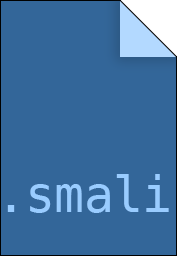
\includegraphics[height=25mm]{resources/images/smali_icon.png}};
    \node[below right] at (9.0,-.15) {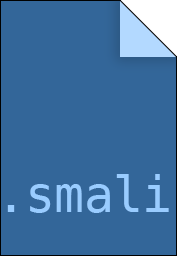
\includegraphics[height=25mm]{resources/images/smali_icon.png}};
    \node[below right] at (9.5,.15) {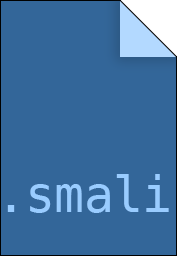
\includegraphics[height=25mm]{resources/images/smali_icon.png}};
    
    \fill[blue, opacity=.25] (3.75,2.25) rectangle (6.75,2.75);
    \node at (5.25,2.5) {\small\textit{\gls{CVE}}};
    \draw[thick,line cap=rect] (3.75,2.25) rectangle (6.75,3.75);
    \draw[thick,line cap=rect] (3.75,2.75) -- (6.75,2.75);
    \draw[xstep=5\textwidth,ystep=.025\textwidth,gray,very thin] (3.75,2.75) grid (6.75,3.75);
    \node[below,align=center] at (5.25,3.8) {\small\textit{Vulnerabilità relative}\\ \textit{ad Android}};
    
    \draw[->,ultra thick] (9.5,2.25) -- (9.5,2.75);
    \draw[->,ultra thick] (9.5,3.25) -- (9.5,4.0);
    \draw[->,ultra thick] (7.0,3.0) -- (9.25,3.0);
    \draw[black,ultra thick,fill=white] (9.5,3.0) circle (.25);
    
    \fill[olive,opacity=.3] (8.0,4.25) rectangle (10.9,4.75);
    \draw[thick,line cap=rect] (8.0,4.25) rectangle (10.9,5.25);;
    \draw[thick,line cap=rect] (8.0,4.75) -- (10.9,4.75);
    \draw[xstep=5\textwidth,ystep=.025\textwidth,gray,very thin] (8.0,4.75) grid (10.9,5.25);
    \node[below,align=center] at (9.45,5.3) {\small\textit{Vulnerabilità \gls{CVE}}\\ \textit{dell'applicazione}};
    \end{tikzpicture}
    \caption{Identificazione delle vulnerabilità utilizzando Apktool}\label{fig:apktool}
\end{figure}
generando in questo modo una cartella al cui interno si trovano anche i file \texttt{.smali}. Il secondo passo consiste nell'individuare all'interno del \gls{CVE} soltanto quelle vulnerabilità nella cui descrizione è presente almeno un nome di file \texttt{.java}. Al momento della stesura della tesi, risultano $43$ elementi che soddisfano questo criterio. A questo punto, per ogni nome di file \texttt{.java} individuato, si controlla se tale nome è presente (sotto forma di stringa) nel codice Smali generato da Apktool (impiegando, ad esempio, il \textit{tool} da linea di comando \texttt{grep}). In caso di esito positivo, l'app in esame risulta soggetta alla vulnerabilità e si può procedere al calcolo di un indice di rischio adoperando il punteggio \gls{CVSS} reperibile nel \gls{NVD}, tramite l'identificativo univoco che caratterizza la vulnerabilità. Esiste tuttavia la possibilità, seppur non considerata in questa tesi, che il codice sorgente dell'applicazione risulti ``offuscato'' e in tal caso non è garantito il funzionamento del metodo proposto. Il termine ``offuscato'' si usa per indicare codice sorgente sintatticamente corretto che però è scritto in maniera volutamente contorta e apparentemente incomprensibile, in modo da rendere il più difficile possibile la comprensione anche da parte dell'utente l'utente più esperto. L'\cref{alg:vulnerability_check} descrive più nel dettaglio la procedura utilizzata per il calcolo di un punteggio di rischio a partire dalla lista \gls{CVE} con le voci relative ad Android.

\begin{algorithm}[!htb]
    \caption{Calcolo di un indice di rischio a partire dalla lista \gls{CVE}}
    \label{alg:vulnerability_check}
    \SetKwData{rischio}{rischio}
    \SetKwData{app}{applicazione}
    \SetKwData{vulnerability}{vulnerabilità}
    \SetKwData{vulnList}{listaVulnerabilità}
    \SetKwData{CVE}{listaCVE}
    \SetKwData{smali}{smali}
    \SetKwData{fileJava}{fileJava}
    \SetKwData{nomeFile}{nomeFile}
    \SetKwData{tmpScore}{tmpScore}
    \SetKwFunction{aggiungi}{aggiungi}
    \SetKwFunction{decompilaApk}{decompilaApk}
    \SetKwFunction{ottieniNomiFileJava}{ottieniNomiFileJava}
    \SetKwFunction{scoreCVSS}{scoreCVSS}
    \SetKwInOut{Input}{Input}\SetKwInOut{Output}{Output}
    \BlankLine
    \Input{Applicazione da analizzare, lista vulnerabilità \gls{CVE}}
    \Output{Indice di rischio per l'applicazione}
    \BlankLine
    $\smali = \decompilaApk{\app}$\;
    \ForEach{\vulnerability in \CVE}
    {
        $\fileJava = \ottieniNomiFileJava{\vulnerability}$\;
        \ForEach{\nomeFile in \fileJava}
        {
            \If{\smali contains \nomeFile}
            {
                \app.\vulnList.\aggiungi{\vulnerability}\;
                \KwSty{continue}
            }
        }     
    }
    \BlankLine
    $\rischio = 0$\;
    \BlankLine
    \ForEach{\vulnerability in \app.\vulnList}
    {
        \tcc{Viene scelto il massimo indice di rischio trovato}
        \tmpScore = \scoreCVSS{\vulnerability}\;
        \If{$\tmpScore > \rischio$}
        {
            $\rischio = \tmpScore$\;
        }  
    }
    \BlankLine
    \Return \rischio\;
\end{algorithm}

\noindent L'approccio appena proposto si rivela tuttavia poco efficace nell'uso pratico, a causa della scarsità di risultati ottenuti. Valutando infatti empiricamente questo metodo su un campione di circa $1~500$ applicazioni del \textit{dataset}, si riesce ad individuare un totale di solamente $3$ vulnerabilità, quindi non si ritiene necessario procedere con l'analisi di ulteriori app. Il fatto di trovare così poche vulnerabilità può anche essere un risultato ragionevole se le applicazioni sono progettate bene e/o non utilizzano componenti di Android afflitti da problematiche di sicurezza; tuttavia l'esiguo numero di riscontri non è sufficiente per permettere di calcolare un punteggio di rischio riferibile in modo generale a tutte le applicazioni, in quanto seguendo questo approccio si avrebbe un indice di rischio nullo per la quasi totalità delle app prese in esame.
\newline

Data la scarsa efficacia di questo primo metodo proposto, si prendono in considerazione due ulteriori criteri per raggiungere lo stesso scopo di costruire un punteggio di rischio, questa volta però concentrandosi sull'\textbf{analisi dei permessi delle applicazioni}:

\begin{itemize}
    \item\textbf{metodo probabilistico} (\cref{sec:probabilistic_method}): si basa direttamente sulla probabilità di richiesta e/o utilizzo di determinati permessi da parte di \textit{malware} e applicazioni benigne, similmente a quanto descritto in \cite{WANG_QUANTITATIVE};
    \item\textbf{metodo basato sul \textit{machine learning}} (\cref{sec:machine_learn_method}): coinvolge l'utilizzo di tecniche di \textit{machine learning} per estrarre un indice di rischio a partire dall'analisi dei permessi di \textit{malware} e applicazioni benigne. Metodologie simili (come ad esempio \cite{DREBIN_DATASET}) sono già presenti in letteratura, però riguardano una classificazione binaria tra \textit{malware} e non \textit{malware}, senza fornire esplicitamente un punteggio di rischio per ogni applicazione esaminata. Questo nuovo metodo proposto nella tesi viene chiamato RiskInDroid.
\end{itemize}



\subsection{Statistiche relative ai permessi}\label{sec:statistiche_permessi}

Prima di procedere illustrando le metodologie basate sull'analisi dei permessi, è opportuno soffermarsi ad esaminare alcune statistiche ad essi relative. In particolare, la motivazione per indagare ulteriormente su questo aspetto delle app nasce dall'osservazione delle differenze che ci sono fra permessi relativi ad applicazioni benigne e quelli collegati ai \textit{malware}.

\begin{figure}[!htb]
    \centering
    \begin{tikzpicture}[x=.09\textwidth,y=-.1\textwidth]
    
    \node[below] at (1.4,-.15) {
\includegraphics[height=25mm]{resources/images/apk_icon.png}};
    \node[below,align=center] at (1.4,1.75) {\small \textit{Applicazione}\\ \textit{Android}};
    
    \node[above] at (2.825,.75) {\small Analisi};
    \draw[->,thick] (2.25,.75) -- (3.5,.75);
    
    \fill[orange,opacity=.3] (3.75,0.0) rectangle (6.75,1.5);
    \node[align=center] at (5.25,.75) {\Large APPROVER\\ \textit{Permission Checker}};
    \draw[thick,line cap=rect,orange] (3.75,0.0) rectangle (6.75,1.5);
    
    \node[above] at (7.625,.75) {\small Risultato};
    \draw[->,thick] (7.0,.75) -- (8.25,.75);
    
    \fill[olive,opacity=.3] (8.5,-.25) rectangle (11.1,.25);
    \node at (9.8,0.0) {\small\textit{Permessi}};
    \draw[thick,line cap=rect] (8.5,-.25) rectangle (11.1,1.8);;
    \draw[thick,line cap=rect] (8.5,.25) -- (11.1,.25);
    \node at (9.8,.5) {\small dichiarati: \{\dots\}};
    \node[align=center] at (9.8,1.0) {\small dichiarati\_e\_usati:\\ \{\dots\}};
    \node at (9.8,1.5) {\small \vdots};
    \node[below] at (9.8,1.85) {\small\textit{File JSON}};
    \end{tikzpicture}
    \caption{Modulo di Approver per l'estrazione dei permessi da un file \texttt{.apk}}\label{fig:permission_checker}
\end{figure}

\noindent Per ottenere i permessi delle applicazioni presenti nel \textit{dataset} viene impiegato il modulo \textit{Permission Checker} di Approver~\cite{APPROVER}. Come visibile nella \cref{fig:permission_checker}, si tratta di un componente che prende in ingresso file di tipo \texttt{.apk} e restituisce in output una lista di permessi (in formato \texttt{JSON}) relativi all'app analizzata.

Nello specifico, il risultato ottenuto dal modulo raggruppa i permessi in $4$ diverse categorie:
\begin{enumerate}
    \item[1)]\textbf{Dichiarati}: permessi richiesti esplicitamente nel file \texttt{AndroidManifest.xml} presente in ogni applicazione per Android. Questa lista è relativamente facile da ricavare anche con altri \textit{tool}, come ad esempio Androguard~\cite{ANDROGUARD};
    \item[2)]\textbf{Dichiarati e utilizzati}: permessi richiesti nel file \texttt{AndroidManifest.xml} che vengono realmente usati dall'applicazione. Per decidere se un permesso è utilizzato o meno, Approver analizza staticamente il \textit{Dalvik bytecode} del file \texttt{classes.dex} contenuto nell'app e determina se vengono invocati metodi che hanno bisogno di permessi per essere eseguiti. Questa lista comprende dunque solo i permessi per cui c'è un riscontro all'interno del \textit{bytecode};
    \item[3)]\textbf{Dichiarati ma non utilizzati}: permessi richiesti soltanto all'interno del file \texttt{AndroidManifest.xml} e per cui non c'è alcun riscontro dentro il \textit{bytecode} dell'applicazione;
    \item[4)]\textbf{Non dichiarati ma utilizzati}: permessi necessari per l'invocazione di metodi all'interno del \textit{bytecode} ma che non sono presenti nel file \texttt{AndroidManifest.xml}.
\end{enumerate}
Esaminando la \cref{fig:p_dichiarati}, si può constatare la differente distribuzione dei permessi dichiarati fra le diverse categorie del \textit{dataset} considerato. È interessante notare come, nel caso dei \textit{malware}, tutti i $15$ permessi della \cref{fig:p_dichiarati:malware} siano richiesti da almeno un quarto delle applicazioni malevole, mentre tale numero scende a $6$ considerando solo i campioni del Google Play Store (\cref{fig:p_dichiarati:goodware}). Si può quindi dedurre che, statisticamente parlando, i \textit{malware} necessitano mediamente di più permessi rispetto al resto delle app. Inoltre, sempre in \cref{fig:p_dichiarati}, si può osservare come le applicazioni provenienti da \textit{store} non ufficiali (\cref{fig:p_dichiarati:aptoide,fig:p_dichiarati:uptodown}) abbiano statistiche che si trovano a metà strada tra \textit{malware} e app benigne, e questo vale non solo per i permessi dichiarati, ma anche per le altre categorie di permessi, i cui grafici sono mostrati nelle \cref{fig:p_dichiarati_usati,fig:p_dichiarati_non_usati,fig:p_non_dichiarati_usati}.
\begin{figure}[!htb]
    \centering
    \begin{subfigure}[t]{.49\textwidth}
        \begin{tikzpicture}[scale=.75]
        \begin{axis}[
        width=.9\textwidth,
        height=1.3\textwidth,
        xmajorgrids,
        grid style={dashed,gray!30},
        xbar,
        y dir=reverse,
        xtick={0,25,...,100},
        ytick=data,
        xmin=0,
        xmax=100,
        y tick label style={align=right,font=\footnotesize\ttfamily},
        enlarge y limits=0.05,
        tick pos=left,
        symbolic y coords={INTERNET,READ\_PHONE\_STATE,ACCESS\_NETWORK\_STATE,WRITE\_EXTERNAL\_STORAGE,SEND\_SMS,ACCESS\_WIFI\_STATE,RECEIVE\_BOOT\_COMPLETED,ACCESS\_COARSE\_LOCATION,RECEIVE\_SMS,WAKE\_LOCK,READ\_SMS,VIBRATE,ACCESS\_FINE\_LOCATION,CHANGE\_WIFI\_STATE,READ\_CONTACTS,}
        ]
        \addplot[red!40!black,fill=red!70!white] coordinates {
            (96.66,INTERNET)
            (90.04,READ\_PHONE\_STATE)
            (70.84,ACCESS\_NETWORK\_STATE)
            (69.79,WRITE\_EXTERNAL\_STORAGE)
            (50.45,SEND\_SMS)
            (48.61,ACCESS\_WIFI\_STATE)
            (46.31,RECEIVE\_BOOT\_COMPLETED)
            (38.03,ACCESS\_COARSE\_LOCATION)
            (37.93,RECEIVE\_SMS)
            (36.99,WAKE\_LOCK)
            (36.72,READ\_SMS)
            (36.57,VIBRATE)
            (36.29,ACCESS\_FINE\_LOCATION)
            (25.96,CHANGE\_WIFI\_STATE)
            (24.66,READ\_CONTACTS)
        };
        \end{axis}
        \end{tikzpicture}
        \captionsetup{justification=centering}
        \caption{Percentuale \textit{malware}}\label{fig:p_dichiarati:malware}
    \end{subfigure}%
    \hfill
    \begin{subfigure}[t]{.49\textwidth}
        \begin{tikzpicture}[scale=.75]
        \begin{axis}[
        width=.9\textwidth,
        height=1.3\textwidth,
        xmajorgrids,
        grid style={dashed,gray!30},
        xbar,
        y dir=reverse,
        xtick={0,25,...,100},
        ytick=data,
        xmin=0,
        xmax=100,
        y tick label style={align=right,font=\footnotesize\ttfamily},
        enlarge y limits=0.05,
        tick pos=left,
        symbolic y coords={INTERNET,ACCESS\_NETWORK\_STATE,WRITE\_EXTERNAL\_STORAGE,ACCESS\_WIFI\_STATE,WAKE\_LOCK,READ\_PHONE\_STATE,VIBRATE,GET\_ACCOUNTS,ACCESS\_COARSE\_LOCATION,READ\_EXTERNAL\_STORAGE,ACCESS\_FINE\_LOCATION,RECEIVE\_BOOT\_COMPLETED,CAMERA,GET\_TASKS,READ\_CONTACTS,}
        ]
        \addplot[green!40!black,fill=green!70!white] coordinates {
            (94.93,INTERNET)
            (89.73,ACCESS\_NETWORK\_STATE)
            (58.06,WRITE\_EXTERNAL\_STORAGE)
            (36.22,ACCESS\_WIFI\_STATE)
            (34.89,WAKE\_LOCK)
            (30.55,READ\_PHONE\_STATE)
            (24.01,VIBRATE)
            (19.67,GET\_ACCOUNTS)
            (18.16,ACCESS\_COARSE\_LOCATION)
            (17.63,READ\_EXTERNAL\_STORAGE)
            (17.11,ACCESS\_FINE\_LOCATION)
            (15.06,RECEIVE\_BOOT\_COMPLETED)
            (10.90,CAMERA)
            (7.92,GET\_TASKS)
            (6.14,READ\_CONTACTS)
        };
        \end{axis}
        \end{tikzpicture}
        \captionsetup{justification=centering}
        \caption{Percentuale app Google Play}\label{fig:p_dichiarati:goodware}
    \end{subfigure}%
    \vspace{.05\textwidth}
    \begin{subfigure}[t]{.49\textwidth}
        \begin{tikzpicture}[scale=.75]
        \begin{axis}[
        width=.9\textwidth,
        height=1.3\textwidth,
        xmajorgrids,
        grid style={dashed,gray!30},
        xbar,
        y dir=reverse,
        xtick={0,25,...,100},
        ytick=data,
        xmin=0,
        xmax=100,
        y tick label style={align=right,font=\footnotesize\ttfamily},
        enlarge y limits=0.05,
        tick pos=left,
        symbolic y coords={INTERNET,ACCESS\_NETWORK\_STATE,WRITE\_EXTERNAL\_STORAGE,WAKE\_LOCK,ACCESS\_WIFI\_STATE,READ\_PHONE\_STATE,VIBRATE,RECEIVE\_BOOT\_COMPLETED,READ\_EXTERNAL\_STORAGE,GET\_ACCOUNTS,ACCESS\_COARSE\_LOCATION,ACCESS\_FINE\_LOCATION,GET\_TASKS,CAMERA,READ\_CONTACTS,}
        ]
        \addplot[orange!40!black,fill=orange!70!white] coordinates {
            (88.84,INTERNET)
            (85.30,ACCESS\_NETWORK\_STATE)
            (69.72,WRITE\_EXTERNAL\_STORAGE)
            (52.02,WAKE\_LOCK)
            (45.77,ACCESS\_WIFI\_STATE)
            (38.64,READ\_PHONE\_STATE)
            (38.10,VIBRATE)
            (30.29,RECEIVE\_BOOT\_COMPLETED)
            (29.59,READ\_EXTERNAL\_STORAGE)
            (29.55,GET\_ACCOUNTS)
            (23.37,ACCESS\_COARSE\_LOCATION)
            (21.66,ACCESS\_FINE\_LOCATION)
            (16.28,GET\_TASKS)
            (15.73,CAMERA)
            (14.97,READ\_CONTACTS)
        };
        \end{axis}
        \end{tikzpicture}
        \captionsetup{justification=centering}
        \caption{Percentuale app Aptoide}\label{fig:p_dichiarati:aptoide}
    \end{subfigure}%
    \hfill
    \begin{subfigure}[t]{.49\textwidth}
        \begin{tikzpicture}[scale=.75]
        \begin{axis}[
        width=.9\textwidth,
        height=1.3\textwidth,
        xmajorgrids,
        grid style={dashed,gray!30},
        xbar,
        y dir=reverse,
        xtick={0,25,...,100},
        ytick=data,
        xmin=0,
        xmax=100,
        y tick label style={align=right,font=\footnotesize\ttfamily},
        enlarge y limits=0.05,
        tick pos=left,
        symbolic y coords={INTERNET,ACCESS\_NETWORK\_STATE,WRITE\_EXTERNAL\_STORAGE,WAKE\_LOCK,ACCESS\_WIFI\_STATE,READ\_PHONE\_STATE,VIBRATE,GET\_ACCOUNTS,READ\_EXTERNAL\_STORAGE,ACCESS\_COARSE\_LOCATION,RECEIVE\_BOOT\_COMPLETED,ACCESS\_FINE\_LOCATION,CAMERA,GET\_TASKS,READ\_CONTACTS,}
        ]
        \addplot[orange!40!black,fill=orange!70!white] coordinates {
            (94.60,INTERNET)
            (90.82,ACCESS\_NETWORK\_STATE)
            (71.75,WRITE\_EXTERNAL\_STORAGE)
            (51.37,WAKE\_LOCK)
            (48.01,ACCESS\_WIFI\_STATE)
            (43.54,READ\_PHONE\_STATE)
            (36.38,VIBRATE)
            (31.02,GET\_ACCOUNTS)
            (25.04,READ\_EXTERNAL\_STORAGE)
            (23.24,ACCESS\_COARSE\_LOCATION)
            (22.19,RECEIVE\_BOOT\_COMPLETED)
            (20.95,ACCESS\_FINE\_LOCATION)
            (14.27,CAMERA)
            (14.02,GET\_TASKS)
            (11.44,READ\_CONTACTS)
        };
        \end{axis}
        \end{tikzpicture}
        \captionsetup{justification=centering}
        \caption{Percentuale app Uptodown}\label{fig:p_dichiarati:uptodown}
    \end{subfigure}%
    \vspace{.01\textwidth}
    \caption{I $15$ permessi più \textbf{dichiarati} dalle applicazioni nel \textit{dataset}}\label{fig:p_dichiarati}
\end{figure}
Ciò potrebbe suggerire che le app di \textit{store} alternativi siano in media meno sicure di quelle provenienti dal Google Play Store, il ché è sensato se si pensa ai maggiori controlli a cui dovrebbero essere sottoposte le applicazioni pubblicate nel Google Play Store.

Non tutti i permessi consentono però di fare una distinzione tra app benigne e maligne. \texttt{INTERNET}, ad esempio, è il permesso più dichiarato (\cref{fig:p_dichiarati}) in tutte le categorie del \textit{dataset} considerato ed è anche quello più utilizzato realmente dalle app (\cref{fig:p_dichiarati_usati}), quindi è impossibile valutare il rischio di un'applicazione considerando solamente questo parametro. Attualmente la maggioranza delle app necessita di una connessione ad Internet:
\begin{figure}[!htb]
    \centering
    \begin{subfigure}[t]{.49\textwidth}
        \begin{tikzpicture}[scale=.75]
        \begin{axis}[
        width=.9\textwidth,
        height=1.3\textwidth,
        xmajorgrids,
        grid style={dashed,gray!30},
        xbar,
        y dir=reverse,
        xtick={0,25,...,100},
        ytick=data,
        xmin=0,
        xmax=100,
        y tick label style={align=right,font=\footnotesize\ttfamily},
        enlarge y limits=0.05,
        tick pos=left,
        symbolic y coords={INTERNET,READ\_PHONE\_STATE,ACCESS\_NETWORK\_STATE,ACCESS\_WIFI\_STATE,ACCESS\_COARSE\_LOCATION,ACCESS\_FINE\_LOCATION,VIBRATE,GET\_TASKS,CHANGE\_WIFI\_STATE,WAKE\_LOCK,WRITE\_EXTERNAL\_STORAGE,RESTART\_PACKAGES,SET\_WALLPAPER,CHANGE\_NETWORK\_STATE,CAMERA,}
        ]
        \addplot[red!40!black,fill=red!70!white] coordinates {
            (76.67,INTERNET)
            (75.65,READ\_PHONE\_STATE)
            (59.43,ACCESS\_NETWORK\_STATE)
            (36.84,ACCESS\_WIFI\_STATE)
            (33.88,ACCESS\_COARSE\_LOCATION)
            (32.06,ACCESS\_FINE\_LOCATION)
            (29.77,VIBRATE)
            (18.61,GET\_TASKS)
            (13.78,CHANGE\_WIFI\_STATE)
            (9.86,WAKE\_LOCK)
            (8.92,WRITE\_EXTERNAL\_STORAGE)
            (6.13,RESTART\_PACKAGES)
            (4.70,SET\_WALLPAPER)
            (3.04,CHANGE\_NETWORK\_STATE)
            (2.77,CAMERA)
        };
        \end{axis}
        \end{tikzpicture}
        \captionsetup{justification=centering}
        \caption{Percentuale \textit{malware}}
    \end{subfigure}%
    \hfill
    \begin{subfigure}[t]{.49\textwidth}
        \begin{tikzpicture}[scale=.75]
        \begin{axis}[
        width=.9\textwidth,
        height=1.3\textwidth,
        xmajorgrids,
        grid style={dashed,gray!30},
        xbar,
        y dir=reverse,
        xtick={0,25,...,100},
        ytick=data,
        xmin=0,
        xmax=100,
        y tick label style={align=right,font=\footnotesize\ttfamily},
        enlarge y limits=0.05,
        tick pos=left,
        symbolic y coords={INTERNET,ACCESS\_NETWORK\_STATE,WAKE\_LOCK,WRITE\_EXTERNAL\_STORAGE,ACCESS\_WIFI\_STATE,VIBRATE,READ\_PHONE\_STATE,ACCESS\_COARSE\_LOCATION,ACCESS\_FINE\_LOCATION,CAMERA,GET\_TASKS,RECORD\_AUDIO,SET\_WALLPAPER,CHANGE\_WIFI\_STATE,WRITE\_SETTINGS,}
        ]
        \addplot[green!40!black,fill=green!70!white] coordinates {
            (91.83,INTERNET)
            (87.62,ACCESS\_NETWORK\_STATE)
            (32.00,WAKE\_LOCK)
            (30.06,WRITE\_EXTERNAL\_STORAGE)
            (24.60,ACCESS\_WIFI\_STATE)
            (23.42,VIBRATE)
            (21.85,READ\_PHONE\_STATE)
            (14.46,ACCESS\_COARSE\_LOCATION)
            (13.67,ACCESS\_FINE\_LOCATION)
            (6.28,CAMERA)
            (5.56,GET\_TASKS)
            (3.12,RECORD\_AUDIO)
            (3.04,SET\_WALLPAPER)
            (2.11,CHANGE\_WIFI\_STATE)
            (1.76,WRITE\_SETTINGS)
        };
        \end{axis}
        \end{tikzpicture}
        \captionsetup{justification=centering}
        \caption{Percentuale app Google Play}
    \end{subfigure}%
    \vspace{.05\textwidth}
    \begin{subfigure}[t]{.49\textwidth}
        \begin{tikzpicture}[scale=.75]
        \begin{axis}[
        width=.9\textwidth,
        height=1.3\textwidth,
        xmajorgrids,
        grid style={dashed,gray!30},
        xbar,
        y dir=reverse,
        xtick={0,25,...,100},
        ytick=data,
        xmin=0,
        xmax=100,
        y tick label style={align=right,font=\footnotesize\ttfamily},
        enlarge y limits=0.05,
        tick pos=left,
        symbolic y coords={INTERNET,ACCESS\_NETWORK\_STATE,WAKE\_LOCK,ACCESS\_WIFI\_STATE,VIBRATE,WRITE\_EXTERNAL\_STORAGE,READ\_PHONE\_STATE,ACCESS\_COARSE\_LOCATION,ACCESS\_FINE\_LOCATION,GET\_TASKS,CHANGE\_WIFI\_STATE,CAMERA,BLUETOOTH,BLUETOOTH\_ADMIN,GET\_ACCOUNTS,}
        ]
        \addplot[orange!40!black,fill=orange!70!white] coordinates {
            (84.45,INTERNET)
            (81.67,ACCESS\_NETWORK\_STATE)
            (44.86,WAKE\_LOCK)
            (36.82,ACCESS\_WIFI\_STATE)
            (36.81,VIBRATE)
            (34.52,WRITE\_EXTERNAL\_STORAGE)
            (32.11,READ\_PHONE\_STATE)
            (19.66,ACCESS\_COARSE\_LOCATION)
            (18.01,ACCESS\_FINE\_LOCATION)
            (13.73,GET\_TASKS)
            (9.55,CHANGE\_WIFI\_STATE)
            (8.64,CAMERA)
            (7.67,BLUETOOTH)
            (4.55,BLUETOOTH\_ADMIN)
            (4.52,GET\_ACCOUNTS)
        };
        \end{axis}
        \end{tikzpicture}
        \captionsetup{justification=centering}
        \caption{Percentuale app Aptoide}
    \end{subfigure}%
    \hfill
    \begin{subfigure}[t]{.49\textwidth}
        \begin{tikzpicture}[scale=.75]
        \begin{axis}[
        width=.9\textwidth,
        height=1.3\textwidth,
        xmajorgrids,
        grid style={dashed,gray!30},
        xbar,
        y dir=reverse,
        xtick={0,25,...,100},
        ytick=data,
        xmin=0,
        xmax=100,
        y tick label style={align=right,font=\footnotesize\ttfamily},
        enlarge y limits=0.05,
        tick pos=left,
        symbolic y coords={INTERNET,ACCESS\_NETWORK\_STATE,WAKE\_LOCK,ACCESS\_WIFI\_STATE,READ\_PHONE\_STATE,VIBRATE,WRITE\_EXTERNAL\_STORAGE,ACCESS\_COARSE\_LOCATION,ACCESS\_FINE\_LOCATION,GET\_TASKS,CAMERA,CHANGE\_WIFI\_STATE,BLUETOOTH,RECORD\_AUDIO,GET\_ACCOUNTS,}
        ]
        \addplot[orange!40!black,fill=orange!70!white] coordinates {
            (91.17,INTERNET)
            (87.97,ACCESS\_NETWORK\_STATE)
            (46.54,WAKE\_LOCK)
            (39.42,ACCESS\_WIFI\_STATE)
            (35.72,READ\_PHONE\_STATE)
            (35.30,VIBRATE)
            (32.52,WRITE\_EXTERNAL\_STORAGE)
            (20.06,ACCESS\_COARSE\_LOCATION)
            (18.13,ACCESS\_FINE\_LOCATION)
            (11.27,GET\_TASKS)
            (8.52,CAMERA)
            (6.39,CHANGE\_WIFI\_STATE)
            (5.70,BLUETOOTH)
            (4.39,RECORD\_AUDIO)
            (3.52,GET\_ACCOUNTS)
        };
        \end{axis}
        \end{tikzpicture}
        \captionsetup{justification=centering}
        \caption{Percentuale app Uptodown}
    \end{subfigure}%
    \vspace{.01\textwidth}
    \captionsetup{justification=centering}
    \caption{I $15$ permessi più \textbf{dichiarati e anche utilizzati} dalle applicazioni nel \textit{dataset}}\label{fig:p_dichiarati_usati}
\end{figure}
applicazioni come quelle di messaggistica istantanea o relative ai \textit{social network} devono accedere alla rete per poter funzionare, ma è sufficiente pensare a giochi per dispositivi mobili che richiedono Internet solo per stilare le classifiche dei punteggi migliori o per mostrare annunci pubblicitari all'utente. Come conseguenza, i permessi riguardanti l'accesso alla rete come \texttt{ACCESS\_NETWORK\_STATE} o \texttt{ACCESS\_WIFI\_STATE} sono anch'essi molto diffusi.

\begin{figure}[!htb]
    \centering
    \begin{subfigure}[t]{.49\textwidth}
        \begin{tikzpicture}[scale=.75]
        \begin{axis}[
        width=.9\textwidth,
        height=1.3\textwidth,
        xmajorgrids,
        grid style={dashed,gray!30},
        xbar,
        y dir=reverse,
        xtick={0,15,30,45,60},
        ytick=data,
        xmin=0,
        xmax=60,
        y tick label style={align=right,font=\footnotesize\ttfamily},
        enlarge y limits=0.05,
        tick pos=left,
        symbolic y coords={WRITE\_EXTERNAL\_STORAGE,SEND\_SMS,RECEIVE\_BOOT\_COMPLETED,RECEIVE\_SMS,READ\_SMS,WAKE\_LOCK,READ\_CONTACTS,INSTALL\_SHORTCUT,INTERNET,READ\_LOGS,SYSTEM\_ALERT\_WINDOW,CALL\_PHONE,READ\_PHONE\_STATE,INSTALL\_PACKAGES,UNINSTALL\_SHORTCUT,}
        ]
        \addplot[red!40!black,fill=red!70!white] coordinates {
            (60.00,WRITE\_EXTERNAL\_STORAGE)
            (50.45,SEND\_SMS)
            (46.31,RECEIVE\_BOOT\_COMPLETED)
            (37.93,RECEIVE\_SMS)
            (36.72,READ\_SMS)
            (27.14,WAKE\_LOCK)
            (24.63,READ\_CONTACTS)
            (22.28,INSTALL\_SHORTCUT)
            (19.99,INTERNET)
            (18.35,READ\_LOGS)
            (16.13,SYSTEM\_ALERT\_WINDOW)
            (14.85,CALL\_PHONE)
            (14.39,READ\_PHONE\_STATE)
            (13.08,INSTALL\_PACKAGES)
            (12.57,UNINSTALL\_SHORTCUT)
        };
        \end{axis}
        \end{tikzpicture}
        \captionsetup{justification=centering}
        \caption{Percentuale \textit{malware}}\label{fig:p_dichiarati_non_usati:malware}
    \end{subfigure}%
    \hfill
    \begin{subfigure}[t]{.49\textwidth}
        \begin{tikzpicture}[scale=.75]
        \begin{axis}[
        width=.9\textwidth,
        height=1.3\textwidth,
        xmajorgrids,
        grid style={dashed,gray!30},
        xbar,
        y dir=reverse,
        xtick={0,15,30,45,60},
        ytick=data,
        xmin=0,
        xmax=60,
        y tick label style={align=right,font=\footnotesize\ttfamily},
        enlarge y limits=0.05,
        tick pos=left,
        symbolic y coords={WRITE\_EXTERNAL\_STORAGE,GET\_ACCOUNTS,READ\_EXTERNAL\_STORAGE,RECEIVE\_BOOT\_COMPLETED,ACCESS\_WIFI\_STATE,READ\_PHONE\_STATE,SYSTEM\_ALERT\_WINDOW,READ\_CONTACTS,CAMERA,CALL\_PHONE,ACCESS\_COARSE\_LOCATION,ACCESS\_FINE\_LOCATION,INTERNET,WRITE\_SETTINGS,INSTALL\_SHORTCUT,}
        ]
        \addplot[green!40!black,fill=green!70!white] coordinates {
            (28.01,WRITE\_EXTERNAL\_STORAGE)
            (18.67,GET\_ACCOUNTS)
            (17.63,READ\_EXTERNAL\_STORAGE)
            (15.06,RECEIVE\_BOOT\_COMPLETED)
            (11.62,ACCESS\_WIFI\_STATE)
            (8.70,READ\_PHONE\_STATE)
            (6.09,SYSTEM\_ALERT\_WINDOW)
            (6.06,READ\_CONTACTS)
            (4.62,CAMERA)
            (4.27,CALL\_PHONE)
            (3.70,ACCESS\_COARSE\_LOCATION)
            (3.44,ACCESS\_FINE\_LOCATION)
            (3.12,INTERNET)
            (3.03,WRITE\_SETTINGS)
            (2.89,INSTALL\_SHORTCUT)
        };
        \end{axis}
        \end{tikzpicture}
        \captionsetup{justification=centering}
        \caption{Percentuale app Google Play}
    \end{subfigure}%
    \vspace{.05\textwidth}
    \begin{subfigure}[t]{.49\textwidth}
        \begin{tikzpicture}[scale=.75]
        \begin{axis}[
        width=.9\textwidth,
        height=1.3\textwidth,
        xmajorgrids,
        grid style={dashed,gray!30},
        xbar,
        y dir=reverse,
        xtick={0,15,30,45,60},
        ytick=data,
        xmin=0,
        xmax=60,
        y tick label style={align=right,font=\footnotesize\ttfamily},
        enlarge y limits=0.05,
        tick pos=left,
        symbolic y coords={WRITE\_EXTERNAL\_STORAGE,RECEIVE\_BOOT\_COMPLETED,READ\_EXTERNAL\_STORAGE,GET\_ACCOUNTS,READ\_CONTACTS,SYSTEM\_ALERT\_WINDOW,WRITE\_SETTINGS,ACCESS\_WIFI\_STATE,INSTALL\_SHORTCUT,CALL\_PHONE,WAKE\_LOCK,CAMERA,CHANGE\_NETWORK\_STATE,READ\_SMS,READ\_PHONE\_STATE,}
        ]
        \addplot[orange!40!black,fill=orange!70!white] coordinates {
            (35.20,WRITE\_EXTERNAL\_STORAGE)
            (30.29,RECEIVE\_BOOT\_COMPLETED)
            (29.59,READ\_EXTERNAL\_STORAGE)
            (25.03,GET\_ACCOUNTS)
            (14.45,READ\_CONTACTS)
            (14.04,SYSTEM\_ALERT\_WINDOW)
            (12.79,WRITE\_SETTINGS)
            (8.95,ACCESS\_WIFI\_STATE)
            (8.60,INSTALL\_SHORTCUT)
            (7.59,CALL\_PHONE)
            (7.15,WAKE\_LOCK)
            (7.09,CAMERA)
            (6.60,CHANGE\_NETWORK\_STATE)
            (6.57,READ\_SMS)
            (6.53,READ\_PHONE\_STATE)
        };
        \end{axis}
        \end{tikzpicture}
        \captionsetup{justification=centering}
        \caption{Percentuale app Aptoide}
    \end{subfigure}%
    \hfill
    \begin{subfigure}[t]{.49\textwidth}
        \begin{tikzpicture}[scale=.75]
        \begin{axis}[
        width=.9\textwidth,
        height=1.3\textwidth,
        xmajorgrids,
        grid style={dashed,gray!30},
        xbar,
        y dir=reverse,
        xtick={0,15,30,45,60},
        ytick=data,
        xmin=0,
        xmax=60,
        y tick label style={align=right,font=\footnotesize\ttfamily},
        enlarge y limits=0.05,
        tick pos=left,
        symbolic y coords={WRITE\_EXTERNAL\_STORAGE,GET\_ACCOUNTS,READ\_EXTERNAL\_STORAGE,RECEIVE\_BOOT\_COMPLETED,READ\_CONTACTS,SYSTEM\_ALERT\_WINDOW,ACCESS\_WIFI\_STATE,READ\_PHONE\_STATE,WRITE\_SETTINGS,INSTALL\_SHORTCUT,CAMERA,RECORD\_AUDIO,CALL\_PHONE,RECEIVE\_SMS,WAKE\_LOCK,}
        ]
        \addplot[orange!40!black,fill=orange!70!white] coordinates {
            (39.23,WRITE\_EXTERNAL\_STORAGE)
            (27.49,GET\_ACCOUNTS)
            (25.04,READ\_EXTERNAL\_STORAGE)
            (22.19,RECEIVE\_BOOT\_COMPLETED)
            (11.24,READ\_CONTACTS)
            (9.92,SYSTEM\_ALERT\_WINDOW)
            (8.59,ACCESS\_WIFI\_STATE)
            (7.82,READ\_PHONE\_STATE)
            (7.76,WRITE\_SETTINGS)
            (7.65,INSTALL\_SHORTCUT)
            (5.75,CAMERA)
            (5.74,RECORD\_AUDIO)
            (5.56,CALL\_PHONE)
            (4.98,RECEIVE\_SMS)
            (4.84,WAKE\_LOCK)
        };
        \end{axis}
        \end{tikzpicture}
        \captionsetup{justification=centering}
        \caption{Percentuale app Uptodown}
    \end{subfigure}%
    \vspace{.01\textwidth}
    \captionsetup{justification=centering}
    \caption{I $15$ permessi più \textbf{dichiarati ma non utilizzati} dalle applicazioni nel \textit{dataset}}\label{fig:p_dichiarati_non_usati}
\end{figure}

\noindent Ci sono poi alcuni permessi come \texttt{READ\_PHONE\_STATE} e \texttt{RECEIVE\_BOOT\_COMPLETED} che sono dichiarati sia dai \textit{malware} che dalle app benigne, ma con percentuali abbastanza differenti, tanto da poter intuire il rischio potenziale di un'applicazione in funzione di tali permessi. Ad esempio, secondo i grafici in \cref{fig:p_dichiarati:malware,fig:p_dichiarati:goodware}, se un'app dichiara \texttt{READ\_PHONE\_STATE}, \texttt{RECEIVE\_BOOT\_COMPLETED} e \texttt{READ\_CONTACTS} allora è statisticamente più probabile che tale app appartenga alla categoria \textit{malware}. La distinzione più significativa fra applicazioni benevole e malevole consiste tuttavia nei permessi relativi agli SMS: infatti, come dimostra la \cref{fig:p_dichiarati:malware}, $3$ dei $15$ permessi più dichiarati dai \textit{malware} riguardano proprio gli SMS, mentre nelle altre categorie del \textit{dataset} in \cref{fig:p_dichiarati} non c'è alcun riferimento al servizio di messaggistica.
\begin{figure}[!htb]
    \centering
    \begin{subfigure}[t]{.49\textwidth}
        \begin{tikzpicture}[scale=.75]
        \begin{axis}[
        width=.9\textwidth,
        height=1.3\textwidth,
        xmajorgrids,
        grid style={dashed,gray!30},
        xbar,
        y dir=reverse,
        xtick={0,15,30,45,60},
        ytick=data,
        xmin=0,
        xmax=60,
        y tick label style={align=right,font=\footnotesize\ttfamily},
        enlarge y limits=0.05,
        tick pos=left,
        symbolic y coords={VIBRATE,WAKE\_LOCK,ACCESS\_COARSE\_LOCATION,ACCESS\_FINE\_LOCATION,CHANGE\_NETWORK\_STATE,KILL\_BACKGROUND\_PRO\dots,ACCESS\_WIFI\_STATE,BLUETOOTH,BLUETOOTH\_ADMIN,CHANGE\_WIFI\_STATE,GET\_TASKS,WRITE\_SETTINGS,READ\_PHONE\_STATE,CAMERA,RECORD\_AUDIO,}
        ]
        \addplot[red!40!black,fill=red!70!white] coordinates {
            (30.55,VIBRATE)
            (24.09,WAKE\_LOCK)
            (12.60,ACCESS\_COARSE\_LOCATION)
            (11.99,ACCESS\_FINE\_LOCATION)
            (9.35,CHANGE\_NETWORK\_STATE)
            (4.46,KILL\_BACKGROUND\_PRO\dots)
            (3.55,ACCESS\_WIFI\_STATE)
            (3.07,BLUETOOTH)
            (3.00,BLUETOOTH\_ADMIN)
            (1.76,CHANGE\_WIFI\_STATE)
            (1.63,GET\_TASKS)
            (1.49,WRITE\_SETTINGS)
            (1.28,READ\_PHONE\_STATE)
            (1.25,CAMERA)
            (1.07,RECORD\_AUDIO)
        };
        \end{axis}
        \end{tikzpicture}
        \captionsetup{justification=centering}
        \caption{Percentuale \textit{malware}}\label{fig:p_non_dichiarati_usati:malware}
    \end{subfigure}%
    \hfill
    \begin{subfigure}[t]{.49\textwidth}
        \begin{tikzpicture}[scale=.75]
        \begin{axis}[
        width=.9\textwidth,
        height=1.3\textwidth,
        xmajorgrids,
        grid style={dashed,gray!30},
        xbar,
        y dir=reverse,
        xtick={0,15,30,45,60},
        ytick=data,
        xmin=0,
        xmax=60,
        y tick label style={align=right,font=\footnotesize\ttfamily},
        enlarge y limits=0.05,
        tick pos=left,
        symbolic y coords={VIBRATE,WAKE\_LOCK,ACCESS\_COARSE\_LOCATION,GET\_TASKS,ACCESS\_FINE\_LOCATION,READ\_PHONE\_STATE,WRITE\_EXTERNAL\_STORAGE,ACCESS\_WIFI\_STATE,BLUETOOTH,CAMERA,CHANGE\_WIFI\_STATE,MODIFY\_AUDIO\_SETTINGS,RECORD\_AUDIO,ACCESS\_NETWORK\_STATE,BLUETOOTH\_ADMIN,}
        ]
        \addplot[green!40!black,fill=green!70!white] coordinates {
            (59.12,VIBRATE)
            (55.41,WAKE\_LOCK)
            (32.95,ACCESS\_COARSE\_LOCATION)
            (32.82,GET\_TASKS)
            (30.40,ACCESS\_FINE\_LOCATION)
            (17.03,READ\_PHONE\_STATE)
            (15.86,WRITE\_EXTERNAL\_STORAGE)
            (11.23,ACCESS\_WIFI\_STATE)
            (7.15,BLUETOOTH)
            (5.11,CAMERA)
            (4.59,CHANGE\_WIFI\_STATE)
            (4.46,MODIFY\_AUDIO\_SETTINGS)
            (4.17,RECORD\_AUDIO)
            (2.98,ACCESS\_NETWORK\_STATE)
            (2.88,BLUETOOTH\_ADMIN)
        };
        \end{axis}
        \end{tikzpicture}
        \captionsetup{justification=centering}
        \caption{Percentuale app Google Play}
    \end{subfigure}%
    \vspace{.05\textwidth}
    \begin{subfigure}[t]{.49\textwidth}
        \begin{tikzpicture}[scale=.75]
        \begin{axis}[
        width=.9\textwidth,
        height=1.3\textwidth,
        xmajorgrids,
        grid style={dashed,gray!30},
        xbar,
        y dir=reverse,
        xtick={0,15,30,45,60},
        ytick=data,
        xmin=0,
        xmax=60,
        y tick label style={align=right,font=\footnotesize\ttfamily},
        enlarge y limits=0.05,
        tick pos=left,
        symbolic y coords={VIBRATE,WAKE\_LOCK,ACCESS\_COARSE\_LOCATION,GET\_TASKS,ACCESS\_FINE\_LOCATION,READ\_PHONE\_STATE,BLUETOOTH,ACCESS\_WIFI\_STATE,WRITE\_EXTERNAL\_STORAGE,MODIFY\_AUDIO\_SETTINGS,CHANGE\_WIFI\_STATE,BLUETOOTH\_ADMIN,CAMERA,BROADCAST\_STICKY,RESTART\_PACKAGES,}
        ]
        \addplot[orange!40!black,fill=orange!70!white] coordinates {
            (42.78,VIBRATE)
            (31.62,WAKE\_LOCK)
            (31.52,ACCESS\_COARSE\_LOCATION)
            (30.17,GET\_TASKS)
            (28.13,ACCESS\_FINE\_LOCATION)
            (18.25,READ\_PHONE\_STATE)
            (11.32,BLUETOOTH)
            (11.11,ACCESS\_WIFI\_STATE)
            (8.92,WRITE\_EXTERNAL\_STORAGE)
            (5.64,MODIFY\_AUDIO\_SETTINGS)
            (4.93,CHANGE\_WIFI\_STATE)
            (4.69,BLUETOOTH\_ADMIN)
            (3.39,CAMERA)
            (3.28,BROADCAST\_STICKY)
            (2.58,RESTART\_PACKAGES)
        };
        \end{axis}
        \end{tikzpicture}
        \captionsetup{justification=centering}
        \caption{Percentuale app Aptoide}
    \end{subfigure}%
    \hfill
    \begin{subfigure}[t]{.49\textwidth}
        \begin{tikzpicture}[scale=.75]
        \begin{axis}[
        width=.9\textwidth,
        height=1.3\textwidth,
        xmajorgrids,
        grid style={dashed,gray!30},
        xbar,
        y dir=reverse,
        xtick={0,15,30,45,60},
        ytick=data,
        xmin=0,
        xmax=60,
        y tick label style={align=right,font=\footnotesize\ttfamily},
        enlarge y limits=0.05,
        tick pos=left,
        symbolic y coords={VIBRATE,ACCESS\_COARSE\_LOCATION,WAKE\_LOCK,ACCESS\_FINE\_LOCATION,GET\_TASKS,READ\_PHONE\_STATE,ACCESS\_WIFI\_STATE,BLUETOOTH,CHANGE\_WIFI\_STATE,WRITE\_EXTERNAL\_STORAGE,MODIFY\_AUDIO\_SETTINGS,CAMERA,BLUETOOTH\_ADMIN,BROADCAST\_STICKY,RECORD\_AUDIO,}
        ]
        \addplot[orange!40!black,fill=orange!70!white] coordinates {
            (47.35,VIBRATE)
            (39.13,ACCESS\_COARSE\_LOCATION)
            (38.95,WAKE\_LOCK)
            (36.91,ACCESS\_FINE\_LOCATION)
            (26.02,GET\_TASKS)
            (18.69,READ\_PHONE\_STATE)
            (12.28,ACCESS\_WIFI\_STATE)
            (11.02,BLUETOOTH)
            (7.24,CHANGE\_WIFI\_STATE)
            (7.12,WRITE\_EXTERNAL\_STORAGE)
            (6.88,MODIFY\_AUDIO\_SETTINGS)
            (6.58,CAMERA)
            (3.86,BLUETOOTH\_ADMIN)
            (3.49,BROADCAST\_STICKY)
            (3.06,RECORD\_AUDIO)
        };
        \end{axis}
        \end{tikzpicture}
        \captionsetup{justification=centering}
        \caption{Percentuale app Uptodown}
    \end{subfigure}%
    \vspace{.01\textwidth}
    \captionsetup{justification=centering}
    \caption{I $15$ permessi più \textbf{utilizzati ma non dichiarati} dalle applicazioni nel \textit{dataset}}\label{fig:p_non_dichiarati_usati}
\end{figure}
Sebbene la maggior parte dei \textit{malware} che richiedono permessi relativi agli SMS in realtà poi non li utilizzano (come testimonia la \cref{fig:p_dichiarati_non_usati:malware}), il fatto che un'app dichiari un permesso riferito agli SMS è comunque un indice di rischio statistico da tenere in considerazione. È infine interessante notare come la categoria dei \textit{malware} sia quella che dichiara più permessi senza poi utilizzarli (\cref{fig:p_dichiarati_non_usati:malware}), quindi è allo stesso tempo anche quella che utilizza meno permessi senza averli dichiarati (\cref{fig:p_non_dichiarati_usati:malware}).



\subsection{Metodo probabilistico}\label{sec:probabilistic_method}

Il metodo probabilistico implementato inizialmente è basato sul lavoro descritto in \cite{WANG_QUANTITATIVE}, in cui viene proposta la seguente formula:
\begin{equation}\label{eq:general_risk}
R_A = \sum_{i} R\left(p_i\right) = \sum_{i} L\left(p_i\right) \times I\left(p_i\right)
\end{equation}
dove $R_A$, il rischio associato all'applicazione $A$, è dato dalla somma dei rischi individuali $R\left(p_i\right)$ di ogni permesso, essendo $L\left(p_i\right)$ e $I\left(p_i\right)$ rispettivamente la probabilità e l'impatto del permesso $p_i$, con $i = 1, 2, \dots, n$ ed $n$ il numero totale di permessi relativi all'applicazione $A$. Si può definire $L\left(p_i\right)$ come la probabilità che l'app $A$ sia maligna nel caso contenga il permesso $p_i$, utilizzando il teorema di Bayes:
\begin{equation}\label{eq:bayes}
L\left(p_i\right) = P\left(A\enspace\text{è malware} \mid p_i\right) = \dfrac{P\left(p_i \mid A\enspace\text{è malware}\right) \times P\left(A\enspace\text{è malware}\right)}{P\left(p_i\right)}
\end{equation}
dove, una volta fissato il \textit{dataset}, $P\left(p_i \mid A\enspace\text{è malware}\right)$ indica la probabilità che un \textit{malware} abbia il permesso $p_i$, $P\left(A\enspace\text{è malware}\right)$ è la probabilità che un'app del \textit{dataset} sia maligna e $P\left(p_i\right)$ indica la probabilità che una qualsiasi applicazione del \textit{dataset} contenga il permesso $p_i$. Ipotizzando, almeno per il momento, che ogni permesso abbia lo stesso impatto $I\left(p_i\right) = 1$, è possibile riscrivere l'\cref{eq:general_risk} per il calcolo di un punteggio di rischio per un'app:

\newlength{\depthofsumsign}
\setlength{\depthofsumsign}{\depthof{$\sum$}}
\newcommand{\nsum}[1][1.9]{
    \mathop{
        \raisebox
        {-#1\depthofsumsign+1\depthofsumsign}
        {\scalebox
            {#1}
            {$\displaystyle\sum$}%
        }
    }
}

\begin{equation}\label{eq:risk_no_impact}
R_A = \nsum_{i} \dfrac{P\left(p_i \mid A\enspace\text{è malware}\right) \times P\left(A\enspace\text{è malware}\right)}{P\left(p_i\right)}
\end{equation}

\noindent A differenza di quanto fatto in \cite{WANG_QUANTITATIVE}, in questa tesi si vuole calcolare un punteggio di rischio percentuale compreso fra $0$ e $100$, quindi il risultato dell'\cref{eq:risk_no_impact} viene normalizzato dividendolo per il numero di permessi $p_i$ relativi all'app $A$ esaminata (moltiplicando infine il tutto per $100$ in modo da ottenere una percentuale). Implementando in codice quanto appena scritto, si ottengono i dati presentati nella \cref{tab:risk_no_impact}, che si riferiscono all'analisi dei soli permessi dichiarati dalle applicazioni nei $3$ set descritti nella \cref{sec:dataset}, usando la tecnica della \textit{k--fold cross validation} dopo aver impostato $k=10$.
\newline

\noindent\textbf{\textit{K--fold cross validation}} \cite{STATISTICAL_INTRO} è un metodo statistico che consiste nel suddividere in modo casuale il \textit{dataset} iniziale in $k$ parti, chiamate \textit{fold}, che abbiano (per quanto possibile) lo stesso numero di elementi. A ogni iterazione su $k$, l'insieme $k$--esimo costituisce il \textit{testing set} (chiamato anche \textit{validation set}) su cui convalidare il modello costruito utilizzando i restanti $k-1$ gruppi, il \textit{training set}. Si calcola quindi un punteggio di accuratezza (percentuale di campioni del \textit{testing set} per cui la classe predetta è uguale a quella reale) per ogni passo $k$--esimo e infine si trova la media di tali $k$ valori. Questo metodo è vantaggioso perché tutti i campioni vengono impiegati sia per allenare sia per testare il modello, riducendo così il problema dell'\textit{overfitting}, che si verifica quando il modello funziona molto bene con i dati usati per fare il \textit{training}, ma i risultati ottenuti sono invece scadenti quando si devono classificare nuovi dati. Il parametro $k$ viene comunemente impostato a $10$, che empiricamente garantisce buoni risultati\footnote{Valore di $k$ consigliato in \cite{CROSS_VALIDATION} e nella documentazione ufficiale della libreria \mbox{\textit{scikit-learn}} consultabile all'indirizzo web \url{http://scikit-learn.org/dev/modules/cross_validation.html}}. Nella \cref{fig:cross_validation} si può osservare graficamente un esempio di \textit{k--fold cross validation} dove si fissa $k=4$.

\begin{figure}[!htb]
    \centering
    \begin{tikzpicture}[x=.06\textwidth,y=-.06\textwidth,scale=.8]
    \filldraw[ultra thick,line cap=rect,fill=orange,fill opacity=.5] (-4.5,0.0) rectangle (-4.0,0.5);
    \filldraw[ultra thick,line cap=rect,fill=blue,fill opacity=.5] (-4.5,1.0) rectangle (-4.0,1.5);
    
    \filldraw[ultra thick,line cap=rect,fill=orange,fill opacity=.5] (0.0,0.0) rectangle (3.0,1.0);
    \filldraw[ultra thick,line cap=rect,fill=blue,fill opacity=.5] (0.0,1.0) rectangle (3.0,2.0);
    \filldraw[ultra thick,line cap=rect,fill=blue,fill opacity=.5] (0.0,2.0) rectangle (3.0,3.0);
    \filldraw[ultra thick,line cap=rect,fill=blue,fill opacity=.5] (0.0,3.0) rectangle (3.0,4.0);
    
    \filldraw[ultra thick,line cap=rect,fill=blue,fill opacity=.5] (4.0,0.0) rectangle (7.0,1.0);
    \filldraw[ultra thick,line cap=rect,fill=orange,fill opacity=.5] (4.0,1.0) rectangle (7.0,2.0);
    \filldraw[ultra thick,line cap=rect,fill=blue,fill opacity=.5] (4.0,2.0) rectangle (7.0,3.0);
    \filldraw[ultra thick,line cap=rect,fill=blue,fill opacity=.5] (4.0,3.0) rectangle (7.0,4.0);
    
    \filldraw[ultra thick,line cap=rect,fill=blue,fill opacity=.5] (8.0,0.0) rectangle (11.0,1.0);
    \filldraw[ultra thick,line cap=rect,fill=blue,fill opacity=.5] (8.0,1.0) rectangle (11.0,2.0);
    \filldraw[ultra thick,line cap=rect,fill=orange,fill opacity=.5] (8.0,2.0) rectangle (11.0,3.0);
    \filldraw[ultra thick,line cap=rect,fill=blue,fill opacity=.5] (8.0,3.0) rectangle (11.0,4.0);
    
    \filldraw[ultra thick,line cap=rect,fill=blue,fill opacity=.5] (12.0,0.0) rectangle (15.0,1.0);
    \filldraw[ultra thick,line cap=rect,fill=blue,fill opacity=.5] (12.0,1.0) rectangle (15.0,2.0);
    \filldraw[ultra thick,line cap=rect,fill=blue,fill opacity=.5] (12.0,2.0) rectangle (15.0,3.0);
    \filldraw[ultra thick,line cap=rect,fill=orange,fill opacity=.5] (12.0,3.0) rectangle (15.0,4.0);
    
    \node[right] at (-4.0,0.25) {\textit{testing set}};
    \node[right] at (-4.0,1.25) {\textit{training set}};
    \foreach \x [count = \i from 0] in {1,...,4} 
    {
        \node[above] at (1.5+4.0*\i,0.0) {\textit{fold} $\x$};
        \draw[->,thick] (1.5+4.0*\i,4.25) -- (1.5+4.0*\i,4.75);
        \node[below] at (1.5+4.0*\i,5.0) {\footnotesize $Accuratezza_\x$};
    }
    
    \node at (7.5,7.0) {$\overline{Accuratezza} = \frac{1}{k} \sum_{i=1}^k Accuratezza_i$};
    \end{tikzpicture}
    \caption{Esempio grafico di \textit{$4$--fold cross validation}}\label{fig:cross_validation}
\end{figure}

\noindent Osservando la \cref{tab:risk_no_impact} si può notare una distinzione abbastanza netta fra i punteggi percentuali generati per i \textit{malware} e quelli per le app benigne; tuttavia è possibile aumentare ulteriormente questa differenza andando ad intervenire sull'impatto $I\left(p_i\right)$ di ogni permesso, finora considerato unitario.

\begin{table}[!htb]
    \renewcommand{\arraystretch}{1.3}
    \centering
    \begin{tabular}{|>{\centering\arraybackslash}m{.18\textwidth}||>{\centering\arraybackslash}m{.1\textwidth}|>{\centering\arraybackslash}m{.1\textwidth}|>{\centering\arraybackslash}m{.1\textwidth}|>{\centering\arraybackslash}m{.1\textwidth}|>{\centering\arraybackslash}m{.1\textwidth}|>{\centering\arraybackslash}m{.1\textwidth}|}
        \hline
        \multirow{2}{*}{\vspace{-10ex}Applicazioni}
        & \multicolumn{2}{c|}{Set~$1$} & \multicolumn{2}{c|}{Set~$2$} & \multicolumn{2}{c|}{Set~$3$}\\\cline{2-7}
        & \rotatebox{90}{\parbox{2cm}{\centering Punteggio medio $\%$}\hspace{.5em}} &
        \rotatebox{90}{\parbox{2cm}{\centering Deviazione standard $\sigma$}\hspace{.5em}} & \rotatebox{90}{\parbox{2cm}{\centering Punteggio medio $\%$}\hspace{.5em}} & \rotatebox{90}{\parbox{2cm}{\centering Deviazione standard $\sigma$}\hspace{.5em}} & \rotatebox{90}{\parbox{2cm}{\centering Punteggio medio $\%$}\hspace{.5em}} & \rotatebox{90}{\parbox{2cm}{\centering Deviazione standard $\sigma$}\hspace{.5em}}\\
        \hline\hline
        \textit{Malware} & $70.16$ & $\hspace{.5em}8.66$ & $70.04$ & $\hspace{.5em}8.64$ & $69.99$ & $\hspace{.5em}8.65$ \\\hline
        Non \textit{malware} & $52.16$ & $11.28$ & $52.07$ & $10.87$ & $51.89$ & $11.48$ \\\hline
    \end{tabular}
    \caption{Indice di rischio normalizzato, con impatto unitario $I\left(p_i\right) = 1$}
    \label{tab:risk_no_impact}
\end{table}



\subsubsection*{Impatto dinamico dei permessi}

In \cite{WANG_QUANTITATIVE} si fissa $I\left(p_i\right) = 1$ per i permessi normali e $I\left(p_i\right) = 1.5$ per quelli \textit{dangerous}. In questo elaborato si decide invece di stabilire l'impatto di un permesso $p_i$ in maniera dinamica e dipendente dal permesso considerato. Si assegna pertanto a $I\left(p_i\right)$ il risultato della divisione fra la probabilità che un \textit{malware} del \textit{dataset} considerato abbia il permesso $p_i$ e la  probabilità che lo stesso permesso $p_i$ sia invece contenuto da un'app benigna:
\begin{equation}\label{eq:impact}
I\left(p_i\right) = \frac{P\left(p_i \mid A\;\text{è malware}\right)}{P\left(p_i \mid A\;\text{non è malware}\right)}
\end{equation}
In questo modo, un permesso richiesto spesso dai \textit{malware} ma che non compare quasi mai nelle applicazioni benigne ha un peso maggiore e influisce molto nel calcolo dell'indice di rischio. Viceversa, i permessi che caratterizzano prevalentemente le app non maligne condizionano poco il risultato finale. L'impatto dinamico attribuito ad ogni permesso dipende dunque dalla qualità del campione statistico utilizzato. Come visto nella \cref{sec:dataset}, in questa tesi si dispone di un ampio \textit{dataset} di applicazioni di cui si conoscono le statistiche relative ai permessi grazie all'analisi effettuata nella \cref{sec:statistiche_permessi}, pertanto è possibile assegnare all'impatto di ogni permesso un valore empiricamente valido. A questo punto, avendo tutti i parametri a disposizione, è possibile utilizzare la formula generale vista nell'\cref{eq:general_risk} (per normalizzare il risultato, ora si divide invece per la somma degli impatti dei singoli permessi). 
\newline

Implementando in codice l'\cref{eq:general_risk} e tenendo conto dell'\cref{eq:impact} si ottengono i risultati visibili nella \cref{tab:risk_and_impact} (lavorando sugli stessi dati della \cref{tab:risk_no_impact}). È interessante notare che, indifferentemente dall'impatto $I\left(p_i\right)$ dei permessi, le statistiche mostrate nelle \cref{tab:risk_no_impact,tab:risk_and_impact}
\begin{table}[!htb]
    \renewcommand{\arraystretch}{1.3}
    \centering
    \begin{tabular}{|>{\centering\arraybackslash}m{.18\textwidth}||>{\centering\arraybackslash}m{.1\textwidth}|>{\centering\arraybackslash}m{.1\textwidth}|>{\centering\arraybackslash}m{.1\textwidth}|>{\centering\arraybackslash}m{.1\textwidth}|>{\centering\arraybackslash}m{.1\textwidth}|>{\centering\arraybackslash}m{.1\textwidth}|}
        \hline
        \multirow{2}{*}{\vspace{-10ex}Applicazioni}
        & \multicolumn{2}{c|}{Set~$1$} & \multicolumn{2}{c|}{Set~$2$} & \multicolumn{2}{c|}{Set~$3$}\\\cline{2-7}
        & \rotatebox{90}{\parbox{2cm}{\centering Punteggio medio $\%$}\hspace{.5em}} &
        \rotatebox{90}{\parbox{2cm}{\centering Deviazione standard $\sigma$}\hspace{.5em}} & \rotatebox{90}{\parbox{2cm}{\centering Punteggio medio $\%$}\hspace{.5em}} & \rotatebox{90}{\parbox{2cm}{\centering Deviazione standard $\sigma$}\hspace{.5em}} & \rotatebox{90}{\parbox{2cm}{\centering Punteggio medio $\%$}\hspace{.5em}} & \rotatebox{90}{\parbox{2cm}{\centering Deviazione standard $\sigma$}\hspace{.5em}}\\
        \hline\hline
        \textit{Malware} & $80.54$ & $10.35$ & $80.42$ & $10.37$ & $80.34$ & $10.39$ \\\hline
        Non \textit{malware} & $56.57$ & $13.65$ & $56.52$ & $13.22$ & $56.20$ & $13.78$ \\\hline
    \end{tabular}
    \caption{Indice di rischio normalizzato, con impatto $I\left(p_i\right) = \frac{P\left(p_i \mid A\;\text{è malware}\right)}{P\left(p_i \mid A\;\text{non è malware}\right)}$}
    \label{tab:risk_and_impact}
\end{table}
sono molto simili per i $3$ set distinti di applicazioni. Questo fatto conferma la validità del metodo utilizzato e permette inoltre di condurre ulteriori prove solamente su un singolo set di app, per poi generalizzare i risultati trovati. Per integrare i dati illustrati nelle \cref{tab:risk_no_impact,tab:risk_and_impact}, la \cref{fig:istogramma} presenta gli istogrammi con i punteggi di rischio nel caso di impatto unitario per ogni permesso e nel caso di utilizzo dell'\cref{eq:impact}. È possibile osservare come i \textit{malware} abbiano mediamente un rischio maggiore rispetto alle applicazioni benigne, anche se è presente una zona dove gli istogrammi di \textit{malware} e non \textit{malware} si sovrappongono e quindi non si può distinguere la categoria a cui appartiene un'app che si trovi in questa regione. Si vede inoltre che esistono alcuni \textit{malware} a rischio massimo ed è presente qualche applicazione a rischio nullo: quest'ultimo fatto si verifica per quelle app che non richiedono alcun permesso. È infine interessante constatare come anche le applicazioni benigne abbiano comunque un rischio quasi sempre maggiore del $40\%$.

% Macro per disegnare i ticks sopra il plot
\makeatletter \newcommand{\pgfplotsdrawaxis}{\pgfplots@draw@axis} \makeatother
\pgfplotsset{axis line on top/.style={
        axis line style=transparent,
        ticklabel style=transparent,
        tick style=transparent,
        axis on top=false,
        after end axis/.append code={
            \pgfplotsset{axis line style=opaque,
                ticklabel style=opaque,
                tick style=opaque,
                grid=none}
            \pgfplotsdrawaxis}
    }
}

\begin{figure}[!htb]
    \centering
        \begin{subfigure}[t]{.49\textwidth}
        \begin{tikzpicture}[scale=.94]
        \begin{axis}[
        axis line on top,
        grid=major,
        grid style={dashed,gray!30},
        area legend,
        xtick={0,20,...,100},
        ytick={0,10,20,30},
        yticklabels={,10,20,30},
        xmin=0,
        xmax=100,
        tick pos=left,
        ymin=0,
        ymax=32.5,
        minor y tick num = 3,
        legend pos=north west,
        legend cell align=left,
        xlabel={\footnotesize \textit{Indice percentuale di rischio}},
        ylabel={\footnotesize \textit{Percentuale di applicazioni}}
        ]
        \legend{\footnotesize\textit{malware},\footnotesize non \textit{malware}};
        % malware
        \addplot+[red!40!black,fill=red!70!white,ybar interval,mark=none,fill opacity=0.8] plot coordinates {
            (0,0.43) (5,0.00) (10,0.00) (15,0.00) (20,0.00) (25,0.00) (30,0.00) (35,0.00) (40,0.01) (45,0.60) (50,1.49) (55,5.32) (60,12.33) (65,29.54) (70,25.59) (75,20.11) (80,2.70) (85,0.24) (90,0.13) (95,1.51) (100,0.00)
        };
        % goodware
        \addplot+[green!40!black,fill=green!70!white,ybar interval,mark=none,fill opacity=0.8] plot coordinates {
            (0,3.19) (5,0.00) (10,0.00) (15,0.00) (20,0.00) (25,0.10) (30,0.01) (35,0.12) (40,3.15) (45,25.29) (50,26.02) (55,27.90) (60,9.57) (65,3.28) (70,0.89) (75,0.34) (80,0.04) (85,0.06) (90,0.01) (95,0.01) (100,0.00)
        };
        \end{axis}
        \end{tikzpicture}
        \caption{Impatto unitario $I\left(p_i\right) = 1$}
    \end{subfigure}%
    \hfill
    \begin{subfigure}[t]{.49\textwidth}
        \begin{tikzpicture}[scale=.94]
        \begin{axis}[
        axis line on top,
        grid=major,
        grid style={dashed,gray!30},
        area legend,
        xtick={0,20,40,...,100},
        ytick={0,10,20,30},
        yticklabels={~~~~},
        xmin=0,
        xmax=100,
        tick pos=left,
        ymin=0,
        ymax=32.5,
        minor y tick num = 3,
        legend pos=north west,
        legend cell align=left,
        xlabel={\footnotesize \textit{Indice percentuale di rischio}}
        ]
        \legend{\footnotesize\textit{malware},\footnotesize non \textit{malware}};
        % malware
        \addplot+[red!40!black,fill=red!70!white,ybar interval,mark=none,fill opacity=0.8] plot coordinates {
            (0,0.43) (5,0.00) (10,0.00) (15,0.00) (20,0.00) (25,0.00) (30,0.00) (35,0.00) (40,0.01) (45,0.54) (50,1.18) (55,0.88) (60,4.20) (65,2.49) (70,12.69) (75,19.14) (80,19.86) (85,27.69) (90,9.26) (95,1.60) (100,0.00)
        };
        % goodware
        \addplot+[green!40!black,fill=green!70!white,ybar interval,mark=none,fill opacity=0.8] plot coordinates {
            (0,3.19) (5,0.00) (10,0.00) (15,0.00) (20,0.00) (25,0.04) (30,0.00) (35,0.00) (40,0.61) (45,18.64) (50,20.25) (55,17.12) (60,21.28) (65,7.17) (70,5.61) (75,3.97) (80,1.37) (85,0.63) (90,0.12) (95,0.01) (100,0.00)
        };
        \end{axis}
        \end{tikzpicture}
        \caption{Impatto $I\left(p_i\right) = \frac{P\left(p_i \mid A\;\text{è malware}\right)}{P\left(p_i \mid A\;\text{non è malware}\right)}$}
    \end{subfigure}%
    \vspace{.01\textwidth}
    \captionsetup{justification=centering}
    \caption{Istogramma dell'indice di rischio normalizzato}\label{fig:istogramma}
\end{figure}

\noindent Per quanto i risultati ottenuti siano interessanti, il metodo di analisi del rischio presentato in questa sezione presenta tuttavia alcuni limiti:
\begin{itemize}
    \item questa metodologia non riesce ad individuare i \textit{malware} che dichiarano pochi o nessun permesso poiché, trattandosi appunto un metodo basato sul numero di permessi, se un'applicazione non richiede alcun permesso allora le verrà assegnato un indice di rischio nullo;
    \item il punteggio di rischio ottenuto impiegando questa tecnica è mediamente alto anche per le applicazioni benigne, per cui ci si aspetterebbe invece di avere indici di rischio situati nella prima metà dell'intervallo di percentuale;
    \item per facilitare il confronto fra diverse applicazioni, in questa tesi si decide di normalizzare il risultato in output dal metodo in modo che ogni app abbia un punteggio di rischio compreso fra due valori fissati (come ad esempio una percentuale da $0$ a $100$). Facendo così, è tuttavia possibile avere casi in cui applicazioni che dichiarano un solo permesso, ma a rischio molto alto (per esempio uno relativo agli SMS - \cref{sec:statistiche_permessi}), risultino più rischiose di altre app che richiedono più permessi ma meno pericolosi.
\end{itemize}



\subsection{Metodo basato sul \textit{machine learning}: RiskInDroid}\label{sec:machine_learn_method}

Per tentare di ovviare ai limiti del metodo probabilistico presentato nella \cref{sec:probabilistic_method}, in questa sezione viene introdotto RiskInDroid, un nuovo metodo per la generazione di un indice di rischio per le applicazioni Android basato su tecniche di \textit{machine learning}. In particolare, viene spiegato come si ottengono i vettori di \textit{feature} a partire dalle app e viene illustrato il processo che ha portato alla decisione di quali classificatori utilizzare per la generazione del punteggio di rischio.

\subsubsection{Estrazione delle \textit{feature}}\label{sec:feature_extraction}

Una volta ottenuti i permessi per tutte le applicazioni nel \textit{dataset} (utilizzando il procedimento descritto nella \cref{sec:statistiche_permessi}), è opportuno riorganizzare i risultati in modo da creare vettori di \textit{feature} confrontabili fra loro e facilmente interpretabili dai più comuni metodi di \textit{machine learning}.

In questo elaborato di laurea, le \textit{feature} vengono costruite in modo simile a quanto fatto in \cite{PERMISSION_FEATURES}: si crea un vettore monodimensionale di capacità $P$, dove a ogni indice corrisponde un determinato permesso (ad esempio la posizione $0$ coincide con il permesso \texttt{CAMERA}, alla posizione $1$ corrisponde \texttt{INTERNET} ecc.). Per ogni applicazione analizzata viene quindi generato un vettore di $P$ \textit{feature} costituito da $1$ e $0$ a seconda che, rispettivamente, l'app contenga o meno il permesso relativo all'indice considerato del vettore. Ad esempio, per una determinata app, se all'indice $0$ corrisponde il permesso \texttt{CAMERA} allora il vettore delle \textit{feature} alla posizione $0$ vale $1$ se tale app contiene il permesso \texttt{CAMERA}, altrimenti vale $0$.

Per la costruzione dei vettori delle \textit{feature} vengono impiegati solamente i permessi disponibili nel sistema operativo Android, la cui lista ufficiale è disponibile online all'indirizzo web \url{http://developer.android.com/reference/android/Manifest.permission.html}. Al momento della stesura della tesi,
\begin{table}[!htb]
    \renewcommand{\arraystretch}{1.3}
    \centering
    \begin{tabular}{|c|c|c||cccc|}
        \hline
        \multicolumn{3}{|r||}{Permessi} & Applicazione $1$ & Applicazione $2$ &\dots& Applicazione $N$\\
        \hline\hline
        \multirow{20}{*}{\rotatebox{90}{\parbox{3cm}{\centering Tutti i permessi}\hspace{.3\normalbaselineskip}}}
        & \multirow{5}{*}{\rotatebox{90}{\parbox{3cm}{\centering Dichiarati}\hspace{.3\normalbaselineskip}}} &
        \texttt{CAMERA} & $0$ & $1$ && $1$ \\
        && \texttt{INTERNET} & $1$ & $1$ && $0$ \\
        && \vdots & \vdots & \vdots & \dots & \vdots \\
        && \texttt{READ\_SMS} & $1$ & $1$ && $0$ \\
        && \texttt{VIBRATE} & $0$ & $1$ && $0$ \\
        \cline{2-7}
        & \multirow{5}{*}{\rotatebox{90}{\parbox{3cm}{\centering Dichiarati e utilizzati}\hspace{.3\normalbaselineskip}}} &
        \texttt{CAMERA} & $0$ & $1$ && $1$ \\
        && \texttt{INTERNET} & $1$ & $1$ && $0$ \\
        && \vdots & \vdots & \vdots & \dots & \vdots \\
        && \texttt{READ\_SMS} & $1$ & $0$ && $0$ \\
        && \texttt{VIBRATE} & $0$ & $0$ && $0$ \\
        \cline{2-7}
        & \multirow{5}{*}{\rotatebox{90}{\parbox{3cm}{\centering Dichiarati ma non utilizzati}\hspace{.3\normalbaselineskip}}} &
        \texttt{CAMERA} & $0$ & $0$ && $0$ \\
        && \texttt{INTERNET} & $0$ & $0$ && $0$ \\
        && \vdots & \vdots & \vdots & \dots & \vdots \\
        && \texttt{READ\_SMS} & $0$ & $1$ && $0$ \\
        && \texttt{VIBRATE} & $0$ & $1$ && $0$ \\
        \cline{2-7}
        & \multirow{5}{*}{\rotatebox{90}{\parbox{3cm}{\centering Non dichiarati ma utilizzati}\hspace{.3\normalbaselineskip}}} &
        \texttt{CAMERA} & $0$ & $0$ && $0$ \\
        && \texttt{INTERNET} & $0$ & $0$ && $0$ \\
        && \vdots & \vdots & \vdots & \dots & \vdots \\
        && \texttt{READ\_SMS} & $0$ & $0$ && $0$ \\
        && \texttt{VIBRATE} & $1$ & $0$ && $1$ \\
        \hline
    \end{tabular}
    \caption{Rappresentazione delle \textit{feature} costruite con i permessi delle applicazioni}
    \label{tab:features}
\end{table}
il numero totale di permessi ammonta a $138$, quindi si decide di impostare la lunghezza dei vettori a $P = 138$. RiskInDroid è progettato per essere un metodo generale e applicabile a qualsiasi applicazione Android, pertanto si sceglie di non aggiungere nei vettori delle \textit{feature} alcun permesso specifico definito dalle app. Includendo infatti come \textit{feature} ogni nuovo permesso definito dalle app analizzate, si otterrebbero vettori di \textit{feature} di lunghezza molto maggiore (sperimentalmente, in questa tesi sono stati individuati in totale $397$ permessi), con un elevato numero di permessi riferiti ad una quantità di app trascurabile rispetto alla grandezza del \textit{dataset} considerato (nelle prove empiriche effettuate sono stati trovati circa $130$ permessi personalizzati dichiarati da meno dello $0.1\%$ dei campioni analizzati).

Per ognuna delle applicazioni esaminate si costruiscono un totale di $5$ vettori di \textit{feature}, di cui il quinto è ridondante poiché costituito dalla sequenza dei primi $4$ (quindi di lunghezza totale $4P$), ma viene creato per comodità e verrà utilizzato nel seguito del lavoro. Gli altri $4$ vettori corrispondono invece alle $4$ categorie di permessi fornite dall'output di Approver: c'è pertanto un vettore di \textit{feature} per i permessi dichiarati, uno per i permessi dichiarati e anche utilizzati, uno per quelli dichiarati ma non utilizzati e infine uno per quelli utilizzati senza essere stati dichiarati. La \cref{tab:features} chiarisce meglio graficamente la struttura dei vettori delle \textit{feature}.



\subsubsection{Classificazione}

Il problema della classificazione \cite{STATISTICAL_INTRO} consiste nell'assegnare le diverse osservazioni sperimentali a una certa categoria fra quelle disponibili e già note. Per gli scopi di questa tesi, le osservazioni sperimentali si riferiscono alle applicazioni Android (in particolare ai loro permessi), mentre le possibili classi sono \texttt{malware} e \texttt{non\_malware}. Si tratta di un metodo supervisionato: è necessario avere una collezione di dati di cui si conosce già la relativa classe di appartenenza. Con tali dati si costruisce un modello per consentire la classificazione accurata di nuovi elementi la cui categoria è inizialmente ignota. L'insieme dei dati di partenza viene chiamato \textit{training set}, e generalmente l'accuratezza del modello viene verificata mediante un \textit{testing set}. La \cref{fig:classificazione} mostra lo schema generale di un classificatore: a partire da un \textit{training set} noto, viene creato un modello che associa a ogni elemento una categoria (in funzione dei suoi attributi o \textit{feature}). Applicando successivamente un \textit{testing set} al classificatore, si può valutare la precisione dello stesso andando a vedere la percentuale di volte in cui la classe predetta dal modello corrisponde a quella realmente presente nel \textit{testing set}. Se i dati di \textit{training} e di \textit{testing} sono stati scelti in maniera opportuna, e l'accuratezza del modello viene ritenuta soddisfacente, si può dare in ingresso al classificatore un elemento la cui categoria è ignota assumendo che la classe predetta sia ragionevolmente uguale a quella reale. In questa tesi si considerano soltanto i classificatori che, oltre ad assegnare una classe, generano in output anche un punteggio di probabilità per quella determinata classe.

\begin{figure}[!htb]
    \centering
    \begin{tikzpicture}[x=.1\textwidth,y=-.08\textwidth]
    
    \node[above] at (1.0,-.25) {\small\textit{Training set}};
    \fill[blue, opacity=.25] (0.0,-.25) rectangle (2.0,0.0);
    \draw[thick,line cap=rect] (0.0,-.25) rectangle (2.0,1.25);
    \draw[thick,line cap=rect] (0.0,0.0) -- (2.0,0.0);
    
    \node[above] at (3.0,.5) {\small Modello};
    \draw[->,thick] (2.25,.5) -- (3.75,.5);
    
    \fill[orange, opacity=.3] (4.0,0.0) rectangle (9.0,1.0);
    \node at (6.5,.5) {\Large CLASSIFICATORE};
    \draw[thick,line cap=rect,orange] (4.0,0.0) rectangle (9.0,1.0);
    
    \node[above] at (5.0,-2.0) {\small\textit{Testing set}};
    \fill[blue,opacity=.25] (4.0,-2.0) rectangle (6.0,-1.75);
    \draw[thick,line cap=rect] (4.0,-2.0) rectangle (6.0,-1.0);;
    \draw[thick,line cap=rect] (4.0,-1.75) -- (6.0,-1.75);
    \draw[->,thick] (5.0,-.75) -- (5.0,-.25);
    
    \node[above] at (8.0,-1.75) {\small Elemento da classificare};
    \draw[thick,line cap=rect] (7.25,-1.75) rectangle (8.75,-1.25);
    \draw[->,thick] (8.0,-1.0) -- (8.0,-.25);
    
    \draw[->,thick] (5.0,1.25) -- (5.0,1.75);
    \node[below,align=center] at (5.0,2.0) {\small Accuratezza del\\ classificatore};
    
    \draw[->,thick] (8.0,1.25) -- (8,1.75);
    \node[below] at (8.0,2.0) {\small Classe dell'elemento};
    
    \draw[->,thick] (8.0,2.5) -- (8.0,2.75);
    \node[draw,dashed] at (8.0,3.25) {\small Probabilità della classe};
    \end{tikzpicture}
    \caption{Rappresentazione schematica di un classificatore}\label{fig:classificazione}
\end{figure}

\noindent Per la creazione di un indice di rischio per le applicazioni viene impiegata la libreria \mbox{\textit{scikit-learn}} per la sua diffusione fra la comunità scientifica, per la relativa semplicità di utilizzo e soprattutto perché contiene molti metodi di classificazione che in output indicano anche la probabilità con cui una determinata classe viene predetta (e non solo il nome della classe stessa). Tale probabilità è una quantità numerica che può essere adoperata per il calcolo di un punteggio di rischio.

La \cref{tab:all_methods} elenca una lista dei classificatori individuati nella libreria \mbox{\textit{scikit-learn}} che contengono una funzione chiamata \texttt{predict\_proba}, la quale permette di avere in output una probabilità per ognuna delle possibili classi del modello. Pertanto, un primo indice di rischio (approfondito in seguito) può essere ottenuto considerando la percentuale riferita alla classe \texttt{malware} quando il classificatore analizza una certa applicazione: più il punteggio è alto, maggiore è la probabilità che tale applicazione sia maligna, quindi il rischio aumenta. Viceversa, un punteggio basso indica che l'applicazione non fa parte della classe \texttt{malware}, pertanto il rischio è minore.

\begin{table}[!htb]
    \renewcommand{\arraystretch}{1.3}
    \centering
    \begin{tabular}{|>{\centering\arraybackslash}m{.48\textwidth}||>{\centering\arraybackslash}m{.09\textwidth}|>{\centering\arraybackslash}m{.09\textwidth}|>{\centering\arraybackslash}m{.09\textwidth}|>{\centering\arraybackslash}m{.09\textwidth}|}
        \hline
        \multirow{2}{*}{Classificatore}
        & \multicolumn{4}{c|}{Accuratezza $\%$}\\\cline{2-5}
        & Set~$1$ & Set~$2$ & Set~$3$ & Media\\
        \hline\hline
        \textit{Support Vector Machines} & $92.99$ & $93.00$ & $92.77$ & $92.92$ \\\hline
        \textit{Gaussian Naive Bayes} & $74.88$ & $74.83$ & $79.61$ & $76.44$ \\\hline
        \textit{Multinomial Naive Bayes} & $90.24$ & $90.01$ & $90.07$ & $90.11$ \\\hline
        \textit{Bernoulli Naive Bayes} & $86.99$ & $87.20$ & $87.03$ & $87.07$ \\\hline
        \textit{Decision Tree} & $94.19$ & $94.46$ & $94.39$ & $94.35$ \\\hline
        \textit{Random Forest} & $95.09$ & $95.25$ & $95.19$ & $95.18$ \\\hline
        \textit{AdaBoost} & $92.63$ & $93.16$ & $92.84$ & $92.88$ \\\hline
        \textit{Gradient Boosting} & $93.08$ & $93.19$ & $93.30$ & $93.19$ \\\hline
        \textit{Stochastic Gradient Descent} & $92.43$ & $92.31$ & $92.36$ & $92.36$ \\\hline
        \textit{Logistic Regression} & $93.10$ & $93.35$ & $93.29$ & $93.25$ \\\hline
        \textit{Logistic Regression CV} & $93.27$ & $93.35$ & $93.31$ & $93.31$ \\\hline
        \textit{Nearest Neighbors} & $78.60$ & $78.79$ & $77.99$ & $78.46$ \\\hline
        \textit{Linear Discriminant Analysis} & $92.46$ & $92.46$ & $92.33$ & $92.42$ \\\hline
        \textit{Quadratic Discriminant Analysis} & $61.89$ & $62.52$ & $67.82$ & $64.08$ \\\hline
        \textit{Multilayer Perceptron Neural Network} & $95.13$ & $95.01$ & $95.16$ & $95.10$ \\\hline  
    \end{tabular}
    \captionsetup{justification=centering}
    \caption{Accuratezza dei classificatori della libreria \mbox{\textit{scikit-learn}} nel classificare le applicazioni appartenenti ai $3$ set descritti nella \cref{sec:dataset}}
    \label{tab:all_methods}
\end{table}

\noindent Per misurare l'affidabilità dei metodi della libreria \mbox{\textit{scikit-learn}} nel classificare fra applicazioni benigne e maligne, vengono effettuate alcune prove per poter valutare empiricamente la percentuale di accuratezza di tali metodi, il cui esito è visibile nella \cref{tab:all_methods}. I risultati presentati sono ottenuti analizzando soltanto i permessi dichiarati dalle applicazioni nei $3$ set descritti nella \cref{sec:dataset} ed usando la tecnica della \textit{k--fold cross validation}, impostando $k=10$ e mantenendo invariati i parametri di default dei classificatori. Si decide di fissare $k=10$ perché sperimentalmente garantisce buoni risultati \cite{CROSS_VALIDATION}; si utilizzano invece i parametri di default dei classificatori poiché si vuole ottenere una comparazione obiettiva dei metodi di classificazione, non influenzata da specifiche configurazioni che potrebbero essere particolarmente adatte alle \textit{feature} impiegate in questo elaborato di laurea.

Come si può notare nella \cref{tab:all_methods}, ci sono alcuni metodi che hanno prestazioni inferiori rispetto agli altri, pertanto vengono scartati a favore di quelli con un'alta percentuale di accuratezza: in questa tesi si imposta empiricamente una soglia minima di precisione a $90\%$ e si continua a lavorare solo con i classificatori che raggiungono questo valore. In alcuni casi, i risultati ottenuti non sono ottimi perché i vettori delle \textit{feature} non sono adatti al tipo di modello scelto: ad esempio, un requisito fondamentale del metodo \textit{Gaussian Naive Bayes} è che i dati in ingresso abbiano una distribuzione di probabilità gaussiana, condizione non verificata dalle \textit{feature} utilizzate in questo elaborato. Altre volte invece la percentuale di accuratezza può essere leggermente aumentata andando ad intervenire sui parametri di costruzione del classificatore, senza avere tuttavia incrementi prestazionali significativi: ad esempio, utilizzando \textit{Nearest Neighbors}, si può modificare il valore di \texttt{n\_neighbors} in ingresso al modello, ottenendo i risultati presentati nella \cref{tab:knn_performance}.

\begin{table}[!htb]
    \renewcommand{\arraystretch}{1.3}
    \centering
    \begin{tabular}{|>{\centering\arraybackslash}m{.3\textwidth}||>{\centering\arraybackslash}m{.1\textwidth}|>{\centering\arraybackslash}m{.1\textwidth}|>{\centering\arraybackslash}m{.1\textwidth}|>{\centering\arraybackslash}m{.1\textwidth}|}
        \hline
        \multirow{2}{*}{Valore di \texttt{n\_neighbors}}
        & \multicolumn{4}{c|}{Accuratezza $\%$}\\\cline{2-5}
        & Set~$1$ & Set~$2$ & Set~$3$ & Media\\
        \hline\hline
        $2$ & $79.85$ & $77.94$ & $81.44$ & $79.75$ \\\hline
        default ($5$) & $78.60$ & $78.79$ & $77.99$ & $78.46$ \\\hline
        $10$ & $82.26$ & $82.74$ & $82.10$ & $82.37$ \\\hline
        $20$ & $81.84$ & $82.46$ & $82.06$ & $82.11$ \\\hline
        $50$ & $82.20$ & $82.92$ & $82.56$ & $82.56$ \\\hline
    \end{tabular}
    \caption{Accuratezza di \textit{Nearest Neighbors} in funzione di \texttt{n\_neighbors}}
    \label{tab:knn_performance}
\end{table}

\noindent Nella \cref{tab:methods_scores} si possono vedere ulteriori informazioni riguardo ai classificatori rimasti dopo l'esclusione di quelli meno efficaci. I risultati sono stati ottenuti sugli stessi $3$ set di applicazioni utilizzati nella \cref{tab:all_methods} ma, per ragioni di spazio, vengono riportati i dati solo dopo aver eseguito la media sui $3$ insiemi. La decisione di mostrare solamente i valori medi è giustificata anche dal fatto che la deviazione standard, che indica la variabilità dei dati rispetto alla media, è sempre minore dell'$1\%$ per ognuno dei risultati presentati in \cref{tab:methods_scores}.

\begin{table}[!htb]
    \renewcommand{\arraystretch}{1.3}
    \centering
    \begin{tabular}{|>{\centering\arraybackslash}m{.3\textwidth}||>{\centering\arraybackslash}m{.1\textwidth}|>{\centering\arraybackslash}m{.1\textwidth}|>{\centering\arraybackslash}m{.1\textwidth}|>{\centering\arraybackslash}m{.1\textwidth}|>{\centering\arraybackslash}m{.1\textwidth}|}
        \hline
        \multirow{2}{*}{\vspace{-10ex}Classificatore}
        & \multirow{2}{*}{\rotatebox{90}{\parbox{2cm}{\centering Accuratezza media $\%$}\hspace{1.2\normalbaselineskip}}}
        & \multicolumn{2}{c|}{\textit{Malware}} & \multicolumn{2}{c|}{Non \textit{malware}}\\\cline{3-6}
        & & \rotatebox{90}{\parbox{2cm}{\centering Punteggio medio $\%$}\hspace{.5em}} & \rotatebox{90}{\parbox{2cm}{\centering Deviazione standard $\sigma$}\hspace{.5em}} & \rotatebox{90}{\parbox{2cm}{\centering Punteggio medio $\%$}\hspace{.5em}} & \rotatebox{90}{\parbox{2cm}{\centering Deviazione standard $\sigma$}\hspace{.5em}}\\
        \hline\hline
        \textit{Support Vector Machines} & $93.05$ & $94.76$ & $\hspace{.5em}8.52$ & $\hspace{.5em}7.71$ & $\hspace{.5em}9.77$ \\\hline
        \textit{Multinomial Naive Bayes} & $88.75$ & $93.52$ & $11.93$ & $12.74$ & $\hspace{.5em}9.79$ \\\hline
        \textit{Decision Tree} & $94.23$ & $99.17$ & $\hspace{.5em}5.10$ & $\hspace{.5em}3.39$ & $\hspace{.5em}6.99$ \\\hline
        \textit{Random Forest} & $95.06$ & $97.23$ & $\hspace{.5em}8.38$ & $\hspace{.5em}5.95$ & $\hspace{.5em}9.62$ \\\hline
        \textit{AdaBoost} & $92.88$ & $52.46$ & $\hspace{.5em}1.66$ & $48.29$ & $\hspace{.5em}1.10$ \\\hline
        \textit{Gradient Boosting} & $93.19$ & $93.77$ & $\hspace{.5em}8.80$ & $\hspace{.5em}9.77$ & $11.26$ \\\hline
        \textit{Stochastic Gradient Descent} & $92.46$ & $95.05$ & $\hspace{.5em}9.29$ & $\hspace{.5em}6.78$ & $10.42$ \\\hline
        \textit{Logistic Regression} & $93.25$ & $94.93$ & $\hspace{.5em}9.40$ & $\hspace{.5em}7.99$ & $10.79$ \\\hline
        \textit{Logistic Regression CV} & $93.31$ & $95.43$ & $\hspace{.5em}9.05$ & $\hspace{.5em}7.48$ & $10.54$ \\\hline
        \textit{Linear Discriminant Analysis} & $92.42$ & $96.55$ & $\hspace{.5em}8.55$ & $\hspace{.5em}3.32$ & $\hspace{.5em}6.96$ \\\hline
        \textit{Multilayer Perceptron Neural Network} & $95.12$ & $98.08$ & $\hspace{.5em}6.64$ & $\hspace{.5em}4.45$ & $\hspace{.5em}7.71$ \\\hline  
    \end{tabular}
    \caption{Punteggi generati dai classificatori}
    \label{tab:methods_scores}
\end{table}

Mentre nella \cref{tab:all_methods} per calcolare la percentuale di accuratezza viene usata una funzione già inclusa nella libreria \mbox{\textit{scikit-learn}} (\texttt{cross\_val\_score}), nella \cref{tab:methods_scores} le statistiche vengono calcolate manualmente. Una volta allenato il modello del classificatore, per ogni elemento del \textit{testing set} analizzato si controlla la probabilità generata per la classe \texttt{malware}: se tale probabilità è maggiore o uguale a $0.5$ ($50\%$) e il campione sotto esame è realmente un \textit{malware}, oppure la probabilità è minore di $0.5$ e l'applicazione non è maligna, allora la predizione del classificatore è esatta. Dividendo quindi il numero di predizioni corrette per il numero totale di elementi nel \textit{testing set}, si ottiene la percentuale di accuratezza. Il motivo per cui quest'ultimo risultato è leggermente diverso fra le \cref{tab:all_methods,tab:methods_scores} è che per calcolare l'output del classificatore la libreria \mbox{\textit{scikit-learn}} ricorre a due metodi differenti, a seconda della necessità o meno di sapere anche la probabilità della classe predetta oltre al nome della classe stessa. Nel primo caso (\cref{tab:all_methods}) viene utilizzata la funzione \texttt{predict}, che in output indica solo il nome della classe, mentre nella \cref{tab:methods_scores} viene impiegata \texttt{predict\_proba}, la quale restituisce anche un valore numerico per la classe predetta. Come si può notare osservando le \cref{tab:all_methods,tab:methods_scores}, le differenze fra i due metodi sono tuttavia esigue nella maggior parte dei casi. Le altre informazioni presenti in \cref{tab:methods_scores} riguardano il punteggio medio generato dai classificatori e la relativa deviazione standard $\sigma$: questi valori sono calcolati facendo riferimento soltanto alle classi predette correttamente, in modo da non introdurre errori dovuti al metodo di classificazione.

Per la creazione di un indice di rischio per le applicazioni si è interessati ai punteggi generati in output dai classificatori (il cui valor medio è riportato nelle colonne $3$ e $5$ della \cref{tab:methods_scores}). Sebbene tutti i metodi di classificazione presentati nella \cref{tab:methods_scores} abbiano una buona accuratezza, non tutti sono adatti per ricavarne un punteggio di rischio affidabile. È possibile infatti eliminare subito \textit{AdaBoost} dalla lista poiché le probabilità che genera in output sono tutte concentrate intorno al $50\%$, impedendo dunque di intuire la pericolosità di un'app se si considera solamente questo dato. In generale, come si può osservare sempre in \cref{tab:methods_scores}, gli altri classificatori restituiscono punteggi prossimi agli estremi dell'intervallo di percentuale, quindi i \textit{malware} tendono ad avere il massimo livello di rischio mentre le applicazioni benigne propendono per un rischio più vicino a $0$, senza avere dunque valori intermedi.
\begin{figure}[!htb]
    \centering
    \begin{subfigure}[t]{.49\textwidth}
        \begin{tikzpicture}[scale=.94]
        \begin{axis}[
        axis line on top,
        grid=major,
        grid style={dashed,gray!30},
        area legend,
        xtick={0,20,...,100},
        ytick={0,25,50,75,100},
        yticklabels={,25,50,75,100},
        xmin=0,
        xmax=100,
        tick pos=left,
        ymin=0,
        ymax=100,
        minor y tick num = 4,
        legend style={at={(0.5,0.97)},anchor=north},
        legend cell align=left,
        xlabel={\footnotesize \textit{Punteggio percentuale di rischio}},
        ylabel={\footnotesize \textit{Percentuale di applicazioni}}
        ]
        \legend{\footnotesize\textit{malware},\footnotesize non \textit{malware}};
        % malware
        \addplot+[red!40!black,fill=red!70!white,ybar interval,mark=none,fill opacity=0.8] plot coordinates {
            (0,3.37) (5,0.30) (10,0.61) (15,0.25) (20,1.15) (25,0.18) (30,0.48) (35,0.15) (40,0.10) (45,0.03) (50,0.48) (55,0.16) (60,0.54) (65,0.24) (70,0.15) (75,0.18) (80,0.13) (85,0.27) (90,0.18) (95,91.05) (100,0.00)
        };
        % goodware
        \addplot+[green!40!black,fill=green!70!white,ybar interval,mark=none,fill opacity=0.8] plot coordinates {
            (0,79.08) (5,3.97) (10,4.55) (15,1.18) (20,3.65) (25,1.00) (30,0.85) (35,0.40) (40,0.15) (45,0.01) (50,0.46) (55,0.09) (60,0.40) (65,0.24) (70,0.04) (75,0.10) (80,0.19) (85,0.03) (90,0.04) (95,3.55) (100,0.00)
        };
        \end{axis}
        \end{tikzpicture}
        \caption{\textit{Decision Tree}}
    \end{subfigure}%
    \hfill
    \begin{subfigure}[t]{.49\textwidth}
        \vspace{.65ex}
        \begin{tikzpicture}[scale=.94]
        \begin{axis}[
        axis line on top,
        grid=major,
        grid style={dashed,gray!30},
        area legend,
        xtick={20,40,...,100},
        ytick={0,25,50,75,100},
        yticklabels={~~~~},
        xmin=0,
        xmax=100,
        tick pos=left,
        ymin=0,
        ymax=100,
        minor y tick num = 4,
        legend style={at={(0.5,0.97)},anchor=north},
        legend cell align=left,
        xlabel={\footnotesize \textit{Punteggio percentuale di rischio}}
        ]
        \legend{\footnotesize\textit{malware},\footnotesize non \textit{malware}};
        % malware
        \addplot+[red!40!black,fill=red!70!white,ybar interval,mark=none,fill opacity=0.8] plot coordinates {
            (0,1.60) (5,0.43) (10,0.92) (15,0.57) (20,0.79) (25,0.55) (30,0.36) (35,0.19) (40,0.36) (45,0.34) (50,0.21) (55,0.42) (60,0.70) (65,0.49) (70,0.40) (75,0.63) (80,0.69) (85,0.94) (90,2.10) (95,87.31) (100,0.00)
        };
        % goodware
        \addplot+[green!40!black,fill=green!70!white,ybar interval,mark=none,fill opacity=0.8] plot coordinates {
            (0,75.37) (5,5.37) (10,5.13) (15,2.76) (20,3.16) (25,1.97) (30,0.76) (35,0.51) (40,0.45) (45,0.48) (50,0.34) (55,0.37) (60,0.52) (65,0.43) (70,0.25) (75,0.34) (80,0.33) (85,0.24) (90,0.42) (95,0.81) (100,0.00)
        };
        \end{axis}
        \end{tikzpicture}
        \caption{\textit{Multilayer Perceptron Neural Network}}
    \end{subfigure}%
    \vspace{.01\textwidth}
    \captionsetup{justification=centering}
    \caption{Istogramma del punteggio percentuale di rischio}\label{fig:hist_dec_tree}
\end{figure}
Tuttavia, metodi di classificazione come \textit{Decision Tree} e \textit{Multilayer Perceptron Neural Network} generano in output probabilità troppo sbilanciate verso gli estremi dell'intervallo di percentuale (come visibile in \cref{fig:hist_dec_tree}), tanto da essere comparabili direttamente a classificatori binari, in quanto, oltre ad indicare se un'app analizzata risulta o meno maligna, non forniscono alcuna informazione aggiuntiva. Di conseguenza è possibile rimuovere tali metodi dall'elenco in \cref{tab:methods_scores}.

\noindent Per quanto riguarda invece \textit{Logistic Regression CV}, si tratta di un classificatore molto simile a \textit{Logistic Regression}, che però implementa un meccanismo interno di \textit{cross validation} con lo scopo di trovare il valore ottimo di un parametro $C$\footnote{\url{http://scikit-learn.org/dev/modules/linear_model.html\#logistic-regression}}, che nel caso della \textit{Logistic Regression} semplice deve essere fornito manualmente (nel caso tale parametro venga omesso, di default si ha $C = 1.0$). Dai dati visibili in \cref{tab:methods_scores} si può osservare che c'è una differenza minima fra i risultati di questi due metodi, pertanto, data la similarità che c'è tra i due classificatori, in questa tesi si decide di proseguire solamente con l'utilizzo di \textit{Logistic Regression}, scartando \textit{Logistic Regression CV}. Un'altra motivazione per questa scelta deriva dal confronto dei tempi di esecuzione: nelle prove empiriche effettuate si è notato che, per fare il \textit{training} del modello, \textit{Logistic Regression} impiega meno di un secondo, mentre per \textit{Logistic Regression CV} sono necessari circa $15$ secondi, senza tuttavia migliorare in modo significativo il risultato finale.

Similmente a quanto fatto per la \cref{tab:all_methods}, in questo elaborato di laurea si stabilisce empiricamente un intervallo limite compreso tra $7\%$ e $95\%$, con lo scopo di escludere i classificatori che restituiscono probabilità troppo sbilanciate verso gli estremi dell'intervallo di percentuale. Applicando questo filtro alla \cref{tab:methods_scores}, rimangono da considerare solamente i seguenti $4$ metodi di classificazione: \textit{Support Vector Machines}, \textit{Multinomial Naive Bayes}, \textit{Gradient Boosting} e \textit{Logistic Regression}. Pertanto, prima di procedere ulteriormente nella trattazione della tesi, è utile soffermarsi a esaminare più nel dettaglio questi $4$ classificatori.



\subsubsection*{\textit{\gls{SVM}}}

Le macchine a vettori di supporto (\gls{SVM}) \cite{STATISTICAL_ELEMENTS} sono un insieme di metodi di apprendimento supervisionato per la risoluzione di problemi di classificazione o di regressione. Si tratta di classificatori binari non probabilistici il cui scopo è la ricerca dell'iperpiano di separazione ottimale fra le due possibili classi all'interno dello spazio delle \textit{feature}, ma è possibile estenderne il funzionamento anche a problemi in cui il numero di classi da predire è maggiore di $2$. Nel caso in cui i dati in input non siano direttamente linearmente separabili, si può ricorrere a funzioni chiamate \textit{kernel} che mappano i dati iniziali in uno spazio di dimensione superiore dove invece è possibile trovare un iperpiano di separazione, pertanto le \gls{SVM} si adattano bene anche a problemi di classificazione non lineare. Le \textit{Support Vector Machines} sono dunque dei classificatori molto potenti che permettono di ricondursi alla classificazione lineare anche quando si devono risolvere problemi molto complessi. Per gli scopi di questo lavoro non è tuttavia necessaria una rigorosa trattazione matematica delle macchine a vettori di supporto, quindi ci si limita a fare un esempio grafico che chiarisca meglio il funzionamento delle \gls{SVM} in un caso di classificazione binaria lineare: come si può vedere in \cref{fig:svm}, in questo semplice esempio è la retta $h$ a dividere le due classi con il margine di separazione massimo.
\begin{figure}[!htb]
    \centering
    \begin{tikzpicture}[>=stealth',scale=1.25]
    \draw [<->,thick] (0,5) node (yaxis) [above] {$y$} |- (5,0) node (xaxis) [right] {$x$};
    
    \draw[very thick] (.5,-.5) -- (5,4);
    
    \filldraw[red,thick] (.5,1.5)  circle (3pt);
    \filldraw[red,thick] (1.5,2.6) circle (3pt);
    \filldraw[red,thick] (1,2.5)   circle (3pt);
    \filldraw[red,thick] (.9,2.1)  circle (3pt);
    \filldraw[red,thick] (.6,1.9)  circle (3pt);
    \filldraw[red,thick] (.5, 2.5) circle (3pt);
    \filldraw[red,thick] (1.5,3)   circle (3pt);
    \filldraw[red,thick] (1.3,3.3) circle (3pt);
    \filldraw[red,thick] (.6,3.2)  circle (3pt);
    \filldraw[very thin] (.5,1.5) -- (1.5,.5);
    \draw[dashed] (-.5,.5) -- (4,5);
    
    \filldraw[blue,thick] (4,1)     circle (3pt); 
    \filldraw[blue,thick] (3.3,.2)  circle (3pt); 
    \filldraw[blue,thick] (4.5,1.2) circle (3pt); 
    \filldraw[blue,thick] (4.5,.5)  circle (3pt); 
    \filldraw[blue,thick] (3.9,.65) circle (3pt); 
    \filldraw[blue,thick] (5,1)     circle (3pt); 
    \filldraw[blue,thick] (3.7,.3)  circle (3pt); 
    \filldraw[blue,thick] (4.1,.3)  circle (3pt);
    \filldraw[very thin] (4,1) -- (3,2);
    \draw[dashed] (1.5,-1.5) -- (6,3);
    
    \node[above right] at (5,4) {$h$};    
    \end{tikzpicture}
    \caption{Esempio grafico di una macchina a vettori di supporto}\label{fig:svm}
\end{figure}



\subsubsection*{\textit{Multinomial Naive Bayes}}

I classificatori bayesiani \cite{BAYESIAN} sono classificatori lineari efficienti e relativamente semplici da realizzare. Si tiene conto del fatto che spesso la relazione tra i valori delle \textit{feature} e quello della classe non è di tipo deterministico; pertanto, per descrivere meglio tale relazione, si ricorre ad un modello probabilistico basato sul teorema di Bayes. In particolare, durante lo svolgimento di questa tesi si utilizzano i classificatori bayesiani naive, ovvero si ritiene che gli attributi degli elementi considerati siano indipendenti fra loro, ipotesi poco realistica che però generalmente si rivela efficace nei problemi pratici. Ci sono più tipi di classificatori bayesiani e si distinguono in base al tipo di distribuzione di probabilità che utilizzano; un'ipotesi molto comune è che le \textit{feature} abbiano una distribuzione di probabilità gaussiana, pertanto il classificatore \textit{Gaussian Naive Bayes} è molto diffuso. Tuttavia, come si può vedere in \cref{tab:all_methods}, in questo elaborato di laurea i risultati migliori si ottengono invece assumendo che le \textit{feature} considerate abbiano una distribuzione probabilistica multinomiale.



\subsubsection*{\textit{Logistic Regression}}

La regressione logistica \cite{PATTERN_RECOGNITION} è un metodo di classificazione che consiste nella creazione di un modello non lineare per studiare la relazione causale esistente tra una variabile dipendente $y$ binaria e una o più variabili indipendenti $x$, che possono assumere valori sia quantitativi sia qualitativi. Si tratta di un problema simile alla regressione lineare multipla, ma in questo caso la variabile $y$ è vincolata ai valori $0$ e $1$, quindi è necessario ricorrere a una funzione particolare detta sigmoide (\cref{fig:logistic}) per rappresentare il legame fra $x$ e $y$ (impiegando la regressione lineare, la variabile $y$ non sarebbe invece limitata ma potrebbe variare fra $(-\infty,+\infty)$).
\begin{figure}[!htb]
    \centering
    \begin{tikzpicture}[scale=.94]
    \begin{axis}[
    xtick={-2,...,2},
    ytick={.5,1},
    xmin=-2,
    xmax=2,
    tick pos=left,
    ymin=0,
    ymax=1.25,
    grid=major,
    grid style={dashed,gray!30},
    xlabel={\footnotesize \textit{Valori osservati di x}},
    ylabel={\footnotesize \textit{Valori previsti di y}}
    ]
    \addplot[domain=-2:2,green!70!black,very thick,samples=500] {1/(1+exp(-3*x))};
    \addplot[domain=-2:2,black,thick,dashed,samples=500] {1};
    \end{axis}
    \end{tikzpicture}
    \caption{Esempio di funzione sigmoide utilizzata nella regressione logistica}\label{fig:logistic}
\end{figure}



\subsubsection*{\textit{Gradient Boosting}}

Il \textit{Gradient Boosting} \cite{BOOSTING} è un metodo \textit{ensemble} di classificazione e di regressione ottenuto dall'accostamento sequenziale di più classificatori. Viene chiamato \textit{ensemble} perché è creato dalla combinazione di più metodi che singolarmente non sono sempre efficaci, ma che insieme garantiscono buoni risultati (in generale come metodo di base si utilizzano gli alberi decisionali). Si tratta di un procedimento iterativo dove ad ogni passo $n$ viene aggiunto un nuovo classificatore di base allo scopo di migliorare il modello complessivo. Considerando come $valore_{predetto} = F(x)$ la funzione del modello di classificazione, tale funzione viene aggiornata ad ogni iterazione allo scopo di migliorare la predizione globale ponendo $F_{n+1}(x) = F_{n}(x) + h_{n}(x)$, dove $h_{n}(x)$ è un classificatore di base creato in modo da minimizzare l'errore di predizione di $F_{n}(x)$. Se si riuscisse a creare un modello perfetto, ad un certo passo $n$ si avrebbe $F_{n}(x) + h_{n}(x) = valore_{atteso}$; riscrivendo $h_{n}(x)$ come $h_{n}(x) = valore_{atteso} - F_{n}(x)$ si può intuire che lo scopo di ogni classificatore di base aggiunto è modellare $valore_{atteso} - F_{n}(x)$ così da ottenere $F_{n+1}(x) = valore_{atteso}$. Definendo la funzione di errore $L(valore_{atteso},F(x)) = \frac{1}{2}(valore_{atteso} - F(x))^2$ e calcolandone il gradiente rispetto ad $F(x)$ si ottiene $F(x) - valore_{atteso}$ che è anche uguale a $-h(x)$, pertanto si ottiene che $F_{n+1}(x) = F_{n}(x) - \nabla L$, quindi ci si è ricondotti a creare un modello utilizzando la tecnica di discesa del gradiente, da cui deriva il nome \textit{Gradient Boosting}. In questo caso si è considerata la funzione di errore $L$ ai minimi quadrati, ma è possibile utilizzare anche altre funzioni di errore (con l'unico vincolo di essere differenziabili).
\newline

A questo punto della tesi si è stabilito empiricamente quali classificatori della libreria \mbox{\textit{scikit-learn}} utilizzare per la creazione di un indice di rischio per le applicazioni Android. Nella \cref{tab:methods_scores} vengono riportati i risultati aggregati ottenuti analizzando i $3$ set di app descritti nella \cref{sec:dataset}; tuttavia, per poter calcolare un punteggio di rischio anche per nuove applicazioni, è necessario prima di tutto allenare il modello di classificazione, e per fare ciò bisogna scegliere quale dei $3$ set impiegare per eseguire il \textit{training}. La \cref{tab:detailed_scores} mostra più nel dettaglio i risultati per ognuno dei $3$ set descritti nella \cref{sec:dataset} (impiegando la \textit{$10$--fold cross validation}), in modo da facilitare la scelta del \textit{training set} da utilizzare nel seguito dell'elaborato di laurea. Come si può infatti notare in \cref{tab:detailed_scores}, le differenze fra i diversi set di ogni classificatore sono pressoché inesistenti, pertanto si decide di fare il \textit{training} dei modelli di classificazione utilizzando solamente il set~$1$, in quanto si è visto empiricamente come i risultati ottenuti siano più generali.

\begin{table}[!htb]
    \renewcommand{\arraystretch}{1.4}
    \centering
    \begin{tabular}{|c|>{\centering\arraybackslash}m{.15\textwidth}||>{\centering\arraybackslash}m{.15\textwidth}|>{\centering\arraybackslash}m{.15\textwidth}|>{\centering\arraybackslash}m{.15\textwidth}|>{\centering\arraybackslash}m{.15\textwidth}|}
        \hline
        \multicolumn{2}{|c||}{\multirow{2}{*}{\vspace{-10ex}Classificatore}}
        & \multicolumn{2}{c|}{\textit{Malware}} & \multicolumn{2}{c|}{Non \textit{malware}}\\\cline{3-6}
        \multicolumn{2}{|c||}{} & \rotatebox{90}{\parbox{2cm}{\centering Punteggio medio $\%$}\hspace{.5em}} & \rotatebox{90}{\parbox{2cm}{\centering Deviazione standard $\sigma$}\hspace{.5em}} & \rotatebox{90}{\parbox{2cm}{\centering Punteggio medio $\%$}\hspace{.5em}} & \rotatebox{90}{\parbox{2cm}{\centering Deviazione standard $\sigma$}\hspace{.5em}}\\
        \hline\hline
        \multirow{4}{*}{\rotatebox{90}{\parbox{3cm}{\centering \textit{Support Vector Machines}}\hspace{.1\normalbaselineskip}}} &
        Set~$1$ & $94.99$ & $\hspace{.5em}8.07$ & $\hspace{.5em}7.77$ & $\hspace{.5em}9.84$ \\\cline{2-6}
        & Set~$2$ & $94.71$ & $\hspace{.5em}8.66$ & $\hspace{.5em}7.72$ & $\hspace{.5em}9.68$ \\\cline{2-6}
        & Set~$3$ & $94.57$ & $\hspace{.5em}8.79$ & $\hspace{.5em}7.66$ & $\hspace{.5em}9.80$ \\\cline{2-6}
        & Media & $94.76$ & $\hspace{.5em}8.52$ & $\hspace{.5em}7.71$ & $\hspace{.5em}9.77$ \\\hline\hline
        
        \multirow{4}{*}{\rotatebox{90}{\parbox{3cm}{\centering \textit{Multinomial Naive Bayes}}\hspace{.3\normalbaselineskip}}} &
        Set~$1$ & $93.33$ & $12.16$ & $12.89$ & $\hspace{.5em}9.93$ \\\cline{2-6}
        & Set~$2$ & $93.51$ & $11.99$ & $12.52$ & $\hspace{.5em}9.70$ \\\cline{2-6}
        & Set~$3$ & $93.73$ & $11.65$ & $12.80$ & $\hspace{.5em}9.74$ \\\cline{2-6}
        & Media & $93.52$ & $11.93$ & $12.74$ & $\hspace{.5em}9.79$ \\\hline\hline
        
        \multirow{4}{*}{\rotatebox{90}{\parbox{3cm}{\centering \textit{Gradient Boosting}}\hspace{.3\normalbaselineskip}}} &
        Set~$1$ & $93.90$ & $\hspace{.5em}8.59$ & $\hspace{.5em}9.84$ & $11.23$ \\\cline{2-6}
        & Set~$2$ & $93.63$ & $\hspace{.5em}8.96$ & $\hspace{.5em}9.66$ & $11.20$ \\\cline{2-6}
        & Set~$3$ & $93.77$ & $\hspace{.5em}8.86$ & $\hspace{.5em}9.80$ & $11.34$ \\\cline{2-6}
        & Media & $93.77$ & $\hspace{.5em}8.80$ & $\hspace{.5em}9.77$ & $11.26$ \\\hline\hline
        
        \multirow{4}{*}{\rotatebox{90}{\parbox{3cm}{\centering \textit{Logistic Regression}}\hspace{.3\normalbaselineskip}}} &
        Set~$1$ & $95.06$ & $\hspace{.5em}9.16$ & $\hspace{.5em}7.96$ & $10.61$ \\\cline{2-6}
        & Set~$2$ & $94.86$ & $\hspace{.5em}9.46$ & $\hspace{.5em}8.01$ & $10.89$ \\\cline{2-6}
        & Set~$3$ & $94.88$ & $\hspace{.5em}9.57$ & $\hspace{.5em}8.00$ & $10.86$ \\\cline{2-6}
        & Media & $94.93$ & $\hspace{.5em}9.40$ & $\hspace{.5em}7.99$ & $10.79$ \\\hline
    \end{tabular}
    \caption{Punteggi dettagliati generati dai classificatori}
    \label{tab:detailed_scores}
\end{table}

Il passo conclusivo per la creazione di un indice di rischio consiste nel combinare i punteggi calcolati dai $4$ classificatori scelti in un unico valore. Per fare ciò si decide di utilizzare la media aritmetica fra le probabilità (riferite alla classe \textit{malware}) generate in output dai $4$ metodi di classificazione considerati. Denotando dunque con $R_A$ il punteggio percentuale di rischio associato ad un'applicazione e con $P_i$ l'output dell'$i$-esimo classificatore (la probabilità relativa alla classe \textit{malware}), si può scrivere l'\cref{eq:risk_mean} per il calcolo del rischio:
\begin{equation}\label{eq:risk_mean}
R_A = \dfrac{1}{N} \sum_{i}^{N} P_i \qquad \text{con} \quad N = 4
\end{equation}
Implementando in codice l'\cref{eq:risk_mean} e applicandola all'insieme di app presenti nel set~$1$, si ottiene l'istogramma presentato in \cref{fig:hist_final:before_rescale}. Nonostante sia meno marcato rispetto a quanto visto in \cref{fig:hist_dec_tree}, si verifica ancora una volta lo sbilanciamento dei punteggi verso gli estremi dell'intervallo di percentuale. Si decide pertanto di ridimensionare l'indice di rischio calcolato precedentemente in modo da ottenere una distribuzione più uniforme, e per fare ciò si impiega una funzione descritta in \cref{fig:logit} ed ispirata alla funzione \texttt{logit} \cite{PATTERN_RECOGNITION}, che in questa tesi viene chiamata ``funzione di ridimensionamento''. La funzione \texttt{logit} è l'inversa della funzione sigmoide vista nel caso della regressione logistica (\cref{fig:logistic}), è definita in $[0,1]$ (perché la variabile dipendente è una probabilità) e può assumere valori in tutto l'intervallo dei numeri reali.

\begin{figure}[!htb]
    \centering
    \begin{subfigure}[t]{.49\textwidth}
        \begin{tikzpicture}[scale=.94]
        \begin{axis}[
        axis line on top,
        grid=major,
        grid style={dashed,gray!30},
        area legend,
        xtick={0,20,...,100},
        ytick={0,25,50,75,100},
        yticklabels={,25,50,75,100},
        xmin=0,
        xmax=100,
        tick pos=left,
        ymin=0,
        ymax=75,
        minor y tick num = 4,
        legend style={at={(0.5,0.97)},anchor=north},
        legend cell align=left,
        xlabel={\footnotesize \textit{Punteggio percentuale di rischio}},
        ylabel={\footnotesize \textit{Percentuale di applicazioni}}
        ]
        \legend{\footnotesize\textit{malware},\footnotesize non \textit{malware}};
        % malware
        \addplot+[red!40!black,fill=red!70!white,ybar interval,mark=none,fill opacity=0.8] plot coordinates {
            (0,0.30) (5,1.09) (10,0.33) (15,0.55) (20,1.82) (25,2.09) (30,0.61) (35,0.72) (40,1.16) (45,0.97) (50,0.55) (55,0.72) (60,0.95) (65,0.97) (70,1.70) (75,3.47) (80,3.15) (85,8.78) (90,7.07) (95,63.01) (100,0.00)
        };
        % goodware
        \addplot+[green!40!black,fill=green!70!white,ybar interval,mark=none,fill opacity=0.8] plot coordinates {
            (0,31.59) (5,35.49) (10,4.38) (15,3.92) (20,5.89) (25,9.69) (30,1.54) (35,1.06) (40,1.00) (45,0.81) (50,0.54) (55,0.51) (60,0.75) (65,0.73) (70,0.19) (75,0.34) (80,0.27) (85,0.33) (90,0.49) (95,0.49) (100,0.00)
        };
        \end{axis}
        \end{tikzpicture}
        \caption{Prima del ridimensionamento}\label{fig:hist_final:before_rescale}
    \end{subfigure}%
    \hfill
    \begin{subfigure}[t]{.49\textwidth}
        \vspace{.65ex}
        \begin{tikzpicture}[scale=.94]
        \begin{axis}[
        axis line on top,
        grid=major,
        grid style={dashed,gray!30},
        area legend,
        xtick={20,40,...,100},
        ytick={0,25,50,75,100},
        yticklabels={~~~~},
        xmin=0,
        xmax=100,
        tick pos=left,
        ymin=0,
        ymax=75,
        minor y tick num = 4,
        legend style={at={(0.5,0.97)},anchor=north},
        legend cell align=left,
        xlabel={\footnotesize \textit{Punteggio percentuale di rischio}}
        ]
        \legend{\footnotesize\textit{malware},\footnotesize non \textit{malware}};
        % malware
        \addplot+[red!40!black,fill=red!70!white,ybar interval,mark=none,fill opacity=0.8] plot coordinates {
            (0,0.00) (5,0.01) (10,0.12) (15,0.21) (20,0.88) (25,0.46) (30,0.54) (35,2.98) (40,1.82) (45,2.43) (50,1.85) (55,2.07) (60,4.70) (65,4.28) (70,8.59) (75,4.29) (80,15.66) (85,6.77) (90,13.75) (95,28.60) (100,0.00)
        };
        % goodware
        \addplot+[green!40!black,fill=green!70!white,ybar interval,mark=none,fill opacity=0.8] plot coordinates {
            (0,3.64) (5,9.35) (10,6.87) (15,16.46) (20,28.28) (25,5.34) (30,5.50) (35,12.94) (40,4.79) (45,2.06) (50,1.65) (55,1.22) (60,0.57) (65,0.27) (70,0.27) (75,0.30) (80,0.22) (85,0.13) (90,0.13) (95,0.00) (100,0.00)
        };
        \end{axis}
        \end{tikzpicture}
        \caption{Dopo il ridimensionamento}\label{fig:hist_final:after_rescale}
    \end{subfigure}%
    \vspace{.01\textwidth}
    \captionsetup{justification=centering}
    \caption{Istogramma dell'indice di rischio finale}\label{fig:hist_final}
\end{figure}
 
\noindent Rispetto alla funzione \texttt{logit}, nella funzione di ridimensionamento utilizzata in questo elaborato i coefficienti sono impostati in modo che la funzione intersechi i punti $(0,0)$, $(50,50)$ e $(100,100)$; in questo caso specifico il dominio della funzione viene considerato $[0,100]$ in quanto si tratta di termini percentuali, di conseguenza anche la funzione assumerà valori in $[0,100]$. L'\cref{eq:logit} descrive la funzione utilizzata e il grafico della stessa è visibile in \cref{fig:logit}.

\begin{equation}\label{eq:logit}
f\left(x\right) = \dfrac{50}{\log\left(101\right)} \log\left(\dfrac{\hspace{1em}1 + x}{101 - x}\right) + 50
\end{equation}

\begin{figure}[!htb]
    \centering
    \begin{tikzpicture}[scale=.94]
    \begin{axis}[
    axis line on top,
    xtick={0,25,...,100},
    ytick={20,40,...,100},
    xmin=0,
    xmax=100,
    ymin=0,
    ymax=100,
    tick pos=left,
    grid=major,
    grid style={dashed,gray!30},
    xlabel={\footnotesize \textit{Indice di rischio attuale}},
    ylabel={\footnotesize \textit{Indice di rischio ridimensionato}},
    samples=1000,
    domain=-1:101,
    ]
    \addplot[red!95!black,very thick] plot (\x, {
            (50 / ln(101)) * (ln(x + 1) - ln(101 - x)) + 50
        });
    \end{axis}
    \end{tikzpicture}
    \caption{Funzione di ridimensionamento dell'indice di rischio}\label{fig:logit}
\end{figure}

\noindent Lo scopo della funzione di ridimensionamento in \cref{fig:logit} è quello di rendere più uniforme la distribuzione della percentuale di rischio presentata in \cref{fig:hist_final:before_rescale}. In particolare, siccome i punteggi generati dai classificatori tendono a raggrupparsi in prossimità degli estremi dell'intervallo di percentuale, la funzione di ridimensionamento ``dilata'' questa regione e ``restringe'' la zona centrale dell'intervallo, dove invece la concentrazione di punteggi è più bassa. In questo modo diventa più facile confrontare le applicazioni ad alto/basso indice di rischio: ad esempio, se per una coppia di app i classificatori generano rispettivamente $99.95\%$ e $99.75\%$, applicando l'\cref{eq:logit} si ottengono invece i punteggi $99.47\%$ e $97.56\%$; pertanto, aumenta la differenza dei valori di rischio e risulta più immediato intuire quale delle due applicazioni sia più rischiosa. Adoperando la funzione descritta dall'\cref{eq:logit} sui dati visualizzabili in \cref{fig:hist_final:before_rescale}, è possibile ottenere una distribuzione più uniforme dei punteggi di rischio, come dimostra il nuovo istogramma in \cref{fig:hist_final:after_rescale}.
\newpage





\section{Risultati}\label{sec:Risultati}

Nella \cref{sec:machine_learn_method} viene presentato RiskInDroid concentrandosi maggiormente sugli aspetti teorici, spiegando le motivazioni per cui sono stati scelti determinati classificatori al posto di altri. In questa sezione si vuole invece testare in maniera più approfondita il metodo RiskInDroid, valutando tutte le categorie di permessi (e non solamente quelli dichiarati come fatto finora) ed estendendo le prove a tutto il \textit{dataset} a disposizione (\cref{tab:APK_dataset}). L'ambiente di test impiegato per eseguire le prove empiriche è descritto in \cref{tab:test_env}.

\begin{table}[!htb]
    \renewcommand{\arraystretch}{1.3}
    \centering
    \begin{tabular}{|>{\centering\arraybackslash}m{.4\textwidth}|>{\centering\arraybackslash}m{.3\textwidth}|}
        \hline
        CPU & Intel i$7$-$3635$QM\\\hline
        RAM & $16$ GB\\\hline
        Sistema Operativo & Windows~$10$\\\hline
        Linguaggio di programmazione & Python $3.5.2$\\\hline
    \end{tabular}
    \caption{Ambiente di test utilizzato per le prove empiriche}
    \label{tab:test_env}
\end{table}

\noindent Dal momento che per RiskInDroid si utilizzano le probabilità generate dai classificatori, è necessario impostare una soglia per poter distinguere i \textit{malware} dal resto delle app. In questa tesi, tale soglia viene fissata a $50\%$ (lo stesso valore usato nella \cref{tab:methods_scores} per determinare l'accuratezza dei classificatori). Il fatto di aver stabilito una soglia di probabilità non va inteso come un metodo generale per la distinzione fra \textit{malware} e applicazioni benigne, che esula dagli scopi di questo elaborato, ma è necessario per poter capire durante i test se un'app, di cui si conosce già la natura, viene classificata in modo corretto. Infatti, nonostante alcune eccezioni, si assume che un \textit{malware} abbia un punteggio di rischio sopra il $50\%$, mentre le applicazioni benigne dovrebbero avere un indice di rischio inferiore a tale soglia. Se dalle prove sperimentali risulta inoltre che ad un alto punteggio di rischio corrisponde, nella maggior parte dei casi, un vero \textit{malware}, allora si ha un'ulteriore conferma della correttezza e dell'affidabilità della metodologia proposta.

Prima di proseguire nell'applicare il metodo RiskInDroid sull'intero \textit{dataset} a disposizione, è interessante valutare la possibilità di ottenere risultati più accurati impiegando tutte le categorie di permessi viste nella \cref{sec:statistiche_permessi}. Finora infatti sono stati utilizzati soltanto i permessi dichiarati per analizzare le prestazioni dei classificatori. Nella \cref{tab:p_accuracy_comparison} vengono quindi mostrate le statistiche di accuratezza relative a tutte le tipologie di permessi, utilizzando le \textit{feature} descritte nella \cref{sec:feature_extraction}. Per ottenere questi risultati si impiega la \textit{$10$--fold cross validation} sull'insieme di applicazioni contenute nel set $1$ (nella \cref{sec:machine_learn_method} si è visto empiricamente che è sufficiente fare le prove su soltanto uno dei $3$ set introdotti nella \cref{sec:dataset}).

\begin{table}[!htb]
    \renewcommand{\arraystretch}{1.3}
    \centering
    \begin{tabular}{|>{\centering\arraybackslash}m{.4\textwidth}||>{\centering\arraybackslash}m{.3\textwidth}|}
        \hline
        Categoria di permessi & Accuratezza $\%$\\
        \hline\hline
        Dichiarati & $92.86$\\\hline
        Dichiarati e utilizzati & $88.39$\\\hline
        Dichiarati ma non utilizzati & $90.91$\\\hline
        Non dichiarati ma utilizzati & $76.60$\\\hline
        Tutti i permessi & $94.94$\\\hline
    \end{tabular}
    \caption{Accuratezza in base alle categorie di permessi}
    \label{tab:p_accuracy_comparison}
\end{table}

\noindent Osservando la \cref{tab:p_accuracy_comparison} si può vedere che l'accuratezza di RiskInDroid dipende soprattutto dai permessi dichiarati; tuttavia, combinando insieme tutte le categorie di permessi, si riesce ad ottenere un valore di accuratezza maggiore rispetto al considerare ogni gruppo singolarmente. Sebbene l'estrazione di altre categorie di permessi sia un'operazione più complessa in confronto al ricavare solamente i permessi dichiarati, nelle prove empiriche effettuate nella \cref{sec:performance} si è notato che ciò non penalizza in modo significativo i tempi di esecuzione di RiskInDroid, se non per quanto riguarda la fase di \textit{training} dei modelli di classificazione (che tuttavia è un'operazione che va eseguita una volta sola). In questa tesi si decide pertanto di utilizzare tutte le categorie di permessi disponibili per la creazione di un indice di rischio, in quanto si è visto empiricamente che in questo modo si ottiene un'accuratezza maggiore.

Una volta definite le categorie di permessi da utilizzare, è necessario stabilire quali e quanti campioni del \textit{dataset} riservare per il \textit{training} dei classificatori. Seguendo la strada intrapresa finora, si decide di impiegare il set $1$ di applicazioni per allenare i modelli di classificazione, ricordando che si tratta di un insieme formato per metà dalla collezione di \textit{malware} presenti nel \textit{dataset} e per l'altra metà da un gruppo di app estratte in modo pseudo-casuale fra le applicazioni scaricate dal Google Play Store, come già visto nella \cref{sec:dataset}. Per valutare sperimentalmente la qualità del \textit{training set} scelto si ricorre alla \textit{$10$--fold cross validation}, i cui risultati sono presentati sotto forma di istogramma nella \cref{fig:hist_all_categ}; in questa circostanza i dati ottenuti vengono mostrati anche all'interno di una matrice di confusione (\cref{tab:confusion_matrix}).

\begin{figure}[!htb]
    \centering
    \begin{tikzpicture}[scale=.94]
    \begin{axis}[
    axis line on top,
    grid=major,
    grid style={dashed,gray!30},
    area legend,
    xtick={0,20,...,100},
    ytick={0,15,30,45},
    yticklabels={,15,30,45},
    xmin=0,
    xmax=100,
    tick pos=left,
    ymin=0,
    ymax=45,
    minor y tick num = 2,
    legend style={at={(0.5,0.97)},anchor=north},
    legend cell align=left,
    xlabel={\footnotesize \textit{Punteggio percentuale di rischio}},
    ylabel={\footnotesize \textit{Percentuale di applicazioni}}
    ]
    \legend{\footnotesize\textit{malware},\footnotesize non \textit{malware}};
    % malware
    \addplot+[red!40!black,fill=red!70!white,ybar interval,mark=none,fill opacity=0.8] plot coordinates {
        (0,0.01) (5,0.07) (10,0.09) (15,0.31) (20,0.28) (25,0.54) (30,0.70) (35,1.12) (40,1.25) (45,1.76) (50,2.33) (55,2.56) (60,1.67) (65,2.88) (70,3.89) (75,5.10) (80,14.37) (85,7.54) (90,14.09) (95,39.42) (100,0.00)
    };
    % goodware
    \addplot+[green!40!black,fill=green!70!white,ybar interval,mark=none,fill opacity=0.8] plot coordinates {
        (0,36.16) (5,11.27) (10,15.55) (15,8.53) (20,5.49) (25,4.28) (30,3.24) (35,5.17) (40,3.38) (45,3.01) (50,1.42) (55,0.63) (60,0.54) (65,0.46) (70,0.28) (75,0.28) (80,0.12) (85,0.13) (90,0.06) (95,0.00) (100,0.00)
    };
    \end{axis}
    \end{tikzpicture}
    \captionsetup{justification=centering}
    \caption{Istogramma dell'indice di rischio generato da RiskInDroid utilizzando tutte le categorie di permessi disponibili}\label{fig:hist_all_categ}
\end{figure}

\begin{table}[!htb]
    \renewcommand{\arraystretch}{2.2}
    \centering
    \begin{tabular}{|c|>{\centering\arraybackslash}m{.2\textwidth}||>{\centering\arraybackslash}m{.2\textwidth}|>{\centering\arraybackslash}m{.2\textwidth}|}
        \hline
        \multicolumn{2}{|c||}{\multirow{2}{*}{\parbox{2.5cm}{\centering App totali: $13~414$}}} & \multicolumn{2}{c|}{Classe predetta}\\\cline{3-4}
        \multicolumn{2}{|c||}{} & \textit{Malware} & Non \textit{malware}\\\hline\hline
        \multirow{2}{*}{\rotatebox{90}{\parbox{2.5cm}{\centering Classe reale}\hspace{.05\normalbaselineskip}}} &
        \textit{Malware} & $6~295$ & $\hspace{.825em}412$ \\\cline{2-4}
        & Non \textit{malware} & $\hspace{.825em}263$ & $6~444$ \\\hline
    \end{tabular}
    \caption{Matrice di confusione del \textit{training set} utilizzato}
    \label{tab:confusion_matrix}
\end{table}

\noindent La \textbf{matrice di confusione} \cite{STATISTICAL_INTRO} è una tabella che descrive in maniera sintetica e intuitiva le prestazioni di un modello di classificazione. In questo caso specifico, sulla diagonale principale è possibile visualizzare il numero di applicazioni classificate in modo corretto: i veri positivi (\textit{malware} correttamente classificati come tali) ed i veri negativi (applicazioni benigne riconosciute correttamente). Nelle altre due celle si trovano invece i falsi positivi (app benigne scambiate per \textit{malware}) ed i falsi negativi (\textit{malware} classificati incorrettamente come applicazioni benigne).
\newline

\noindent Dalla \cref{tab:confusion_matrix} è possibile calcolare alcuni indici statistici per ottenere una valutazione empirica dell'affidabilità di RiskInDroid e del \textit{training set} selezionato:
\begin{itemize}
    \item\textbf{Accuratezza} $= 0.949$, denota il rapporto fra il numero di applicazioni correttamente classificate (sia maligne sia benigne) e il numero totale di app analizzate;
    \item\textbf{Precisione} $= 0.959$, indica la proporzione fra i \textit{malware}  classificati correttamente e il totale di applicazioni classificate come \textit{malware};
    \item\textbf{\textit{Recall}} $= 0.938$, esprime il rapporto fra i \textit{malware}  classificati correttamente e il totale di \textit{malware} esaminati.
\end{itemize}
Visti i buoni risultati ottenuti empiricamente per il \textit{training set} considerato, è possibile procedere con il calcolo del punteggio di rischio per tutte le applicazioni presenti nel \textit{dataset} a disposizione (il \textit{training set} è stato fissato, pertanto il resto delle app costituiscono il \textit{testing set}). Nella \cref{fig:hist_google_play} si può quindi vedere l'istogramma con gli indici di rischio per la collezione completa di app provenienti dal Google Play Store (ad esclusione del gruppo di applicazioni già incluse nel \textit{training set}).

\begin{figure}[!htb]
    \centering
    \begin{tikzpicture}
    \begin{axis}[
    axis line on top,
    grid=major,
    grid style={dashed,gray!30},
    area legend,
    xtick={0,20,...,100},
    ytick={0,15,30,45},
    yticklabels={,15,30,45},
    xmin=0,
    xmax=100,
    tick pos=left,
    ymin=0,
    ymax=45,
    minor y tick num = 2,
    xlabel={\footnotesize \textit{Punteggio percentuale di rischio}},
    ylabel={\footnotesize \textit{Percentuale di applicazioni}}
    ]
    % google play
    \addplot+[green!40!black,fill=green!70!white,ybar interval,mark=none,fill opacity=0.8] plot coordinates {
        (0,35.95) (5,11.27) (10,16.60) (15,8.34) (20,5.28) (25,3.88) (30,3.14) (35,5.08) (40,3.70) (45,2.69) (50,1.27) (55,0.72) (60,0.66) (65,0.40) (70,0.26) (75,0.26) (80,0.23) (85,0.13) (90,0.10) (95,0.05) (100,0.00)
    };
    \end{axis}
    \end{tikzpicture}
    \captionsetup{justification=centering}
    \caption{Istogramma dell'indice di rischio generato da RiskInDroid per le app provenienti dal Google Play Store}\label{fig:hist_google_play}
\end{figure}

\begin{figure}[!htb]
    \centering    
    \begin{subfigure}[t]{.49\textwidth}
        \begin{tikzpicture}[scale=.94]
        \begin{axis}[
        axis line on top,
        grid=major,
        grid style={dashed,gray!30},
        area legend,
        xtick={0,20,...,100},
        ytick={0,10,...,40},
        yticklabels={,10,20,30},
        xmin=0,
        xmax=100,
        tick pos=left,
        ymin=0,
        ymax=32.5,
        minor y tick num = 4,
        xlabel={\footnotesize \textit{Punteggio percentuale di rischio}},
        ylabel={\footnotesize \textit{Percentuale di applicazioni}}
        ]
        % aptoide
        \addplot+[orange!40!black,fill=orange!70!white,ybar interval,mark=none,fill opacity=0.8] plot coordinates {
            (0,29.97) (5,10.72) (10,8.56) (15,6.57) (20,5.06) (25,4.57) (30,4.02) (35,10.34) (40,6.72) (45,4.58) (50,3.07) (55,1.59) (60,1.09) (65,1.00) (70,0.53) (75,0.57) (80,0.38) (85,0.37) (90,0.17) (95,0.09) (100,0.00)
        };
        \end{axis}
        \end{tikzpicture}
        \caption{Aptoide}
    \end{subfigure}%
    \hfill
    \begin{subfigure}[t]{.49\textwidth}
        \begin{tikzpicture}[scale=.94]
        \begin{axis}[
        axis line on top,
        grid=major,
        grid style={dashed,gray!30},
        area legend,
        xtick={0,20,...,100},
        ytick={0,10,...,40},
        yticklabels={~~~~},
        xmin=0,
        xmax=100,
        tick pos=left,
        ymin=0,
        ymax=32.5,
        minor y tick num = 4,
        xlabel={\footnotesize \textit{Punteggio percentuale di rischio}}
        ]
        % uptodown
        \addplot+[orange!40!black,fill=orange!70!white,ybar interval,mark=none,fill opacity=0.8] plot coordinates {
            (0,27.58) (5,12.95) (10,14.46) (15,7.23) (20,5.71) (25,4.39) (30,4.21) (35,6.68) (40,5.42) (45,3.72) (50,2.67) (55,1.64) (60,0.80) (65,0.80) (70,0.34) (75,0.53) (80,0.32) (85,0.22) (90,0.15) (95,0.17) (100,0.00)
        };
        \end{axis}
        \end{tikzpicture}
        \caption{Uptodown}
    \end{subfigure}%
    \vspace{.01\textwidth}
    \captionsetup{justification=centering}
    \caption{Istogramma dell'indice di rischio generato da RiskInDroid per le app provenienti da fonti non ufficiali}\label{fig:hist_unofficial}
\end{figure}

\noindent Nella \cref{fig:hist_unofficial} è possibile invece osservare l'istogramma con i punteggi di rischio per i campioni del \textit{dataset} provenienti da canali non ufficiali. A prescindere dalla fonte da cui sono state scaricate le applicazioni, esaminando gli istogrammi in \cref{fig:hist_google_play,fig:hist_unofficial} si può intuire che si tratta perlopiù di app non malevole.



\subsection{Confronto con antivirus}

Per concludere l'analisi sperimentale di RiskInDroid, si vuole determinare la reale pericolosità delle applicazioni per le quali è stato individuato un punteggio di rischio alto da parte del metodo proposto in questa tesi. Per fare ciò, si raccolgono tutte le app del \textit{dataset} per le quali RiskInDroid ha calcolato un valore di rischio superiore al $75\%$, e si analizzano successivamente con una suite di più di $50$ antivirus online resa disponibile gratuitamente da VirusTotal\footnote{\url{http://www.virustotal.com}}. Lo scopo di questo esperimento è di valutare il livello di affidabilità del metodo di analisi di RiskInDroid rispetto ai tradizionali approcci \textit{signature-based} generalmente utilizzati dagli antivirus. I risultati ottenuti da questo confronto sono mostrati nella \cref{tab:perm_vs_signature}, dove il numero di \textit{flag} indica quanti degli antivirus interrogati da VirusTotal
\begin{table}[!htb]
    \renewcommand{\arraystretch}{1.3}
    \centering
    \begin{tabular}{|>{\centering\arraybackslash}m{.225\textwidth}||>{\centering\arraybackslash}m{.21\textwidth}|c|c|c|}
        \hline
        Fonte applicazioni & \# app con rischio $\geq 75\%$ & \# \textit{flag} $\geq 1$ & \# \textit{flag} $\geq 3$ & \# \textit{flag} $\geq 15$\\
        \hline\hline
        Google Play Store & $792$ & $173$ & $101$ & $30$\\\hline
        Aptoide & $110$ & $\hspace{.5em}22$ & $\hspace{.5em}11$ & $\hspace{.5em}5$\\\hline
        Uptodown & $103$ & $\hspace{.5em}29$ & $\hspace{.5em}14$ & $\hspace{.5em}4$\\\hline
    \end{tabular}
    \captionsetup{justification=centering}
    \caption{Statistiche ottenute esaminando le applicazioni più rischiose con VirusTotal}
    \label{tab:perm_vs_signature}
\end{table}
riconoscono una determinata applicazione come \textit{malware}. I numeri riferiti alle app provenienti dal Google Play Store sono più alti perché le applicazioni esaminate provengono in massima parte da tale \textit{store}; se però, al posto di considerare i valori assoluti, si calcolano invece le percentuali, si ottengono risultati simili per tutte le categorie di applicazioni presenti nella \cref{tab:perm_vs_signature}. In particolare, si può notare che in ogni categoria circa il $4\%$ delle app più rischiose sia riconosciuto come \textit{malware} da almeno $15$ antivirus. In conclusione, tale analisi comparativa suggerisce che l'approccio adottato da RiskInDroid sia promettente e che l'indice di rischio generato sia affidabile, in quanto fra le applicazioni più rischiose sono stati individuati alcuni \textit{malware} da un buon numero di antivirus.

Dal momento che RiskInDroid risulta empiricamente attendibile per la definizione del rischio delle applicazioni Android, un suo possibile impiego consiste nel valutare potenziali \textit{zero-day malware}. Si tratta di \textit{malware} che sfruttano vulnerabilità di sistema non ancora note pubblicamente o che agiscono con modalità mai viste in precedenza; in questo caso gli approcci tradizionali \textit{signature-based} sono poco efficaci in quanto il loro funzionamento si basa sulla conoscenza pregressa delle ``firme'' di \textit{malware} già noti, e pertanto non riescono ad individuare i \textit{malware} che presentano comportamenti nuovi rispetto a quelli già conosciuti.



\subsection{Considerazioni sui tempi di esecuzione}\label{sec:performance}

Finora è stata valutata solamente la qualità e l'affidabilità dei risultati generati da RiskInDroid. Per avere un quadro più completo, in questa sezione si analizzano invece le prestazioni di RiskInDroid per quanto riguarda i tempi di esecuzione, utilizzando la configurazione hardware/software descritta nella \cref{tab:test_env}.

Il funzionamento di RiskInDroid può essere suddiviso in $3$ passi principali: estrazione dei vettori di \textit{feature} dalle applicazioni, \textit{training} dei modelli di classificazione (eseguito una volta sola) e calcolo effettivo del punteggio di rischio delle app che si vogliono analizzare. Come già visto più in dettaglio nella \cref{sec:statistiche_permessi}, per l'estrazione delle \textit{feature} viene impiegato il modulo \textit{Permission Checker} di Approver. Nella \cref{tab:perm_check_perf} è possibile osservare i tempi medi e la deviazione standard ($\sigma$) in millisecondi necessari per ottenere le \textit{feature} delle applicazioni nel \textit{dataset}, sia nel caso in cui si decida di estrarre tutte le categorie di permessi, effettuando dunque un'analisi statica completa,
\begin{table}[!htb]
    \renewcommand{\arraystretch}{1.3}
    \centering
    \begin{tabular}{|>{\centering\arraybackslash}m{.3\textwidth}||>{\centering\arraybackslash}m{.125\textwidth}|>{\centering\arraybackslash}m{.125\textwidth}|>{\centering\arraybackslash}m{.125\textwidth}|>{\centering\arraybackslash}m{.125\textwidth}|}
        \hline
        \multirow{2}{*}{Fonte applicazioni}
        & \multicolumn{2}{c|}{Analisi completa} & \multicolumn{2}{c|}{Analisi del \textit{Manifest}}\\\cline{2-5}
        & $t_{medio}$ [ms] & $\sigma$ [ms] & $t_{medio}$ [ms] & $\sigma$ [ms]\\
        \hline\hline
        Raccolta \textit{malware} & $\hspace{.5em}47$ & $40$ & $30$ & $16$\\\hline
        Google Play Store & $\hspace{.5em}99$ & $62$ & $34$ & $17$\\\hline
        Aptoide & $127$ & $91$ & $50$ & $43$\\\hline
        Uptodown & $127$ & $88$ & $47$ & $40$\\\hline
    \end{tabular}
    \captionsetup{justification=centering}
    \caption{Prestazioni del modulo \textit{Permission Checker} di Approver}
    \label{tab:perm_check_perf}
\end{table}
sia quando si vogliono invece ottenere solamente i permessi dichiarati nel \textit{Manifest} (ovvero nel file \texttt{AndroidManifest.xml} contenuto in ogni app). Le differenze nelle statistiche delle categorie di applicazioni sono imputabili alla diversa grandezza media delle app (le app più grandi richiedono infatti più tempo per essere esaminate), tuttavia si tratta di valori trascurabili se comparati al tempo medio necessario per fare il \textit{training} dei modelli di classificazione utilizzati da RiskInDroid, visualizzati nella \cref{tab:training_perf} (tali valori corrispondono alla media dei risultati ottenuti dopo $10$ iterazioni). In questo caso si può notare come, usando tutte le categorie di permessi, ci sia un divario abbastanza marcato rispetto all'utilizzare soltanto i permessi dichiarati. Questa differenza è dovuta soprattutto alle \textit{Support Vector Machines} e al \textit{Gradient Boosting}, in quanto gli altri due classificatori (\textit{Multinomial Naive Bayes} e \textit{Logistic Regression}) hanno prestazioni quasi uguali a prescindere dal numero di permessi impiegati.

\begin{table}[!htb]
    \renewcommand{\arraystretch}{1.3}
    \centering
    \begin{tabular}{|>{\centering\arraybackslash}m{.3\textwidth}||>{\centering\arraybackslash}m{.125\textwidth}|>{\centering\arraybackslash}m{.125\textwidth}|>{\centering\arraybackslash}m{.125\textwidth}|>{\centering\arraybackslash}m{.125\textwidth}|}
        \hline
        \multirow{2}{*}{Classificatore}
        & \multicolumn{2}{c|}{Permessi dichiarati} & \multicolumn{2}{c|}{Tutti i permessi}\\\cline{2-5}
        & $t_{medio}$ [ms] & $\sigma$ [ms] & $t_{medio}$ [ms] & $\sigma$ [ms]\\
        \hline\hline
        \textit{Support Vector Machines} & $43~460$ & $60$ & $\hspace{.5em}97~170$ & $870$\\\hline
        \textit{Multinomial Naive Bayes} & $\hspace{1.825em}32$ & $\hspace{.5em}4$ & $\hspace{2.325em}53$ & $\hspace{.5em}11$\\\hline
        \textit{Gradient Boosting} & $\hspace{.5em}5~620$ & $52$ & $\hspace{.5em}21~806$ & $403$\\\hline
        \textit{Logistic Regression} & $\hspace{1.825em}81$ & $\hspace{.5em}9$ & $\hspace{1.825em}188$ & $\hspace{.5em}11$\\\hline\hline
        Totale & $49~193$ & $67$ & $119~220$ & $890$\\\hline
    \end{tabular}
    \captionsetup{justification=centering}
    \caption{Tempo medio necessario per il \textit{training} dei classificatori di RiskInDroid}
    \label{tab:training_perf}
\end{table}

\noindent Una volta eseguito il \textit{training} dei classificatori presenti in RiskInDroid ed assumendo di aver già estratto le \textit{feature} dalle applicazioni, calcolare i punteggi di rischio delle app risulta un'operazione estremamente veloce, nell'ordine di pochi millisecondi, pertanto non si ritiene necessario riportare tali valori in una tabella. È importante sottolineare il fatto che il \textit{training} dei modelli di classificazione è un'operazione che va eseguita una volta sola prima di analizzare le applicazioni, pertanto è accettabile avere dei tempi di esecuzione in questa fase se poi si ottengono benefici in termini di accuratezza ed affidabilità.
\newpage





\section{Conclusioni e Sviluppi Futuri}\label{sec:Conclusioni}

In questa tesi è stato proposto RiskInDroid, un metodo per la generazione di un punteggio di rischio per le applicazioni Android basato su tecniche di \textit{machine learning}. Prima però di definire RiskInDroid sono state valutate altre due tecniche con lo scopo di calcolare un indice di rischio per le app. In un primo momento, si è tentato di sviluppare un metodo che sfruttasse le informazioni sulle vulnerabilità presenti nell'elenco \gls{CVE}, che però si è rivelato inefficace a causa di un esiguo numero di riscontri ottenuti. Come alternativa, si è provato a migliorare una metodologia già esistente nella letteratura scientifica \cite{WANG_QUANTITATIVE}, ottenendo risultati interessanti ma che presentavano ancora alcune caratteristiche indesiderate (come ad esempio un punteggio di rischio mediamente alto anche per le applicazioni benigne). Dal momento che nessuno dei due metodi proposti inizialmente si è rivelato soddisfacente, è stato ideato un nuovo approccio per il calcolo del rischio, a cui è stato attribuito il nome RiskInDroid. Una estensiva analisi sperimentale su $116~541$ app benigne e $6~707$ \textit{malware} ha dimostrato che RiskInDroid permette di calcolare indici di rischio affidabili con buone prestazioni computazionali.

L'obiettivo di creare un metodo per l'analisi del rischio delle applicazioni Android è stato quindi raggiunto: si è riusciti ad implementare un punteggio di rischio che risulta corretto (la percentuale di accuratezza ha un valore alto, $94.9\%$) ed affidabile (sono state eseguite prove empiriche su un campione statistico significativo formato da un totale di $123~248$ elementi). Uno dei fattori che hanno contribuito all'ottenimento di questi risultati è l'aver considerato tutte le categorie di permessi riferiti alle app e non solo quelli dichiarati, come invece è stato fatto nella maggior parte degli altri lavori presenti nella letteratura scientifica. Sebbene lo scopo di questo lavoro non sia la classificazione binaria di \textit{malware}, le app benigne esaminate per cui risultava un alto valore di rischio sono state analizzate anche tramite il portale VirusTotal, per determinare se esiste una qualche relazione tra un punteggio di rischio elevato e la reale pericolosità di un'applicazione. Si è scoperto che l'indice calcolato da RiskInDroid è ragionevole, in quanto fra le app (in teoria benigne) a rischio maggiore erano presenti alcuni \textit{malware}. Tuttavia, RiskInDroid non è un classificatore binario di \textit{malware} e non deve essere impiegato in tale contesto. Infine, è importante osservare che un'app non deve necessariamente appartenere alla categoria \textit{malware} per essere rischiosa. Si consideri, ad esempio, un'applicazione legittima per la gestione dei contatti e degli SMS, che necessita inoltre di una connessione ad Internet per fornire alcune funzionalità aggiuntive; pur non trattandosi di un \textit{malware}, tale applicazione è comunque una potenziale minaccia per la privacy dell'utente, pertanto è lecito aspettarsi che abbia un elevato punteggio di rischio.

Come già accennato nell'introduzione, il problema della sicurezza del sistema Android è molto attuale, pertanto è bene disporre di quanti più strumenti possibile che aiutino a salvaguardare l'utente dalle applicazioni pericolose. In questo contesto si inserisce anche Approver, un prodotto software professionale per l'analisi completa delle applicazioni mobili, sviluppato da Talos S.r.l.s (\url{http://www.talos-security.com/}) e che verrà rilasciato ad ottobre $2016$. RiskInDroid si presenta dunque come un \textit{tool} implementato e funzionante per il calcolo di un punteggio di rischio per le applicazioni Android, che verrà integrato come componente di Approver, di cui utilizza già il modulo \textit{Permission Checker} per ottenere i vettori di \textit{feature} delle applicazioni esaminate.



\subsection*{Sviluppi Futuri}

Questo elaborato di laurea lascia spazio ad ulteriori approfondimenti e sviluppi futuri. Si è visto che i vettori di \textit{feature} utilizzati per allenare i modelli di classificazione permettono di ottenere empiricamente buoni risultati; si potrebbe dunque provare a migliorare ulteriormente tali risultati aumentando il numero e il tipo di \textit{feature} impiegate, aggiungendo altre informazioni (oltre ai permessi) ricavate dall'analisi statica delle app, come ad esempio le chiamate ad \acrshort{API} sospette oppure indirizzi di rete e \acrshort{URL} individuati nel codice sorgente decompilato delle applicazioni (analogamente a quanto fatto in \cite{DREBIN_DATASET}). Potrebbe infine essere interessante esplorare anche tecniche di analisi dinamica (come ad esempio Crowdroid \cite{CROWDROID}), non prese in considerazione durante lo svolgimento di questa tesi, al fine di ottenere un metodo ancora più preciso ed affidabile di calcolo del rischio per le applicazioni Android.





\newpage
\cleardoublepage
\phantomsection
\addcontentsline{toc}{section}{Bibliografia}
\bibliography{resources/bibliografia.bib}
\end{document}
